%%%%%%%%%%%%%%%%%%%%%%%%%%%%%%%%%
% 6CCS3PRJ Final Year Individual Project Report
% luke.day@kcl.ac.uk
%%%%%%%%%%%%%%%%%%%%%%%%%%%%%%%%%
\documentclass[11pt]{informatics-report}
\usepackage{color}
\usepackage{hyperref}
\usepackage[justification=Centering]{caption}
\usepackage{float}
\usepackage{graphicx}
\graphicspath{Images/}
\newcommand{\link}[1]{\href{#1}{#1}}
\usepackage[square,sort,comma,numbers]{natbib} %References

%%%%%%%%%%%%%%%%%%%%%%%%%%%%%%%%%
% Front Matter - project title, name, supervisor name and date
%%%%%%%%%%%%%%%%%%%%%%%%%%%%%%%%%
\title{6CCS3PRJ Final Year\\\vspace{0.2cm}Individual Project Report Title}
\author{Zishan Rahman}
\studentID{20071291}
\supervisor{Senir Dinar}

\date{\today}

\abstractFile{FrontMatter/abstract.tex}
\ackFile{FrontMatter/acknowledgements.tex} %Remove line if you do not want acknowledgements

\begin{document}
\createFrontMatter
\onehalfspacing
\tableofcontents
\doublespacing

%%%%%%%%%%%%%%%%%%%%%%%%%%%%%%%%%
% Report Content
%%%%%%%%%%%%%%%%%%%%%%%%%%%%%%%%%
% You can write each chapter directly here or in a separate .tex file and use the include command.

\chapter{Introduction}
%This is one of the most important components of the report. It should begin with a clear statement of what the project is about so that the nature and scope of the project can be understood by a lay reader. It should summarise everything that you set out to achieve, provide a clear summary of the project's background and relevance to other work, and give pointers to the remaining sections of the report, which will contain the bulk of the technical material.

Procedural Content Generation, or PCG, refers to the use of algorithms and programming in lieu of human handiwork to design and implement various contents in video games, such as levels, terrains, trees and cities. A PCG algorithm is ontogenetic when it tries to produce a foreseeable end result as it goes along. For this project, I will be implementing several well-known ontogenetic algorithms in a basic 3D walking simulator game, using the open-source Godot game engine, and then comparing how each algorithm carries out the creation of levels in said game.

\section{Report Structure}

\chapter{Background} \label{Background}
%The background should set the project into context by motivating the subject matter and relating it to existing published work. The background will include a critical evaluation of the existing literature in the area in which your project work is based and should lead the reader to understand how your work is motivated by and related to existing work.

For my BSc individual project, I will be researching procedural content generation (PCG) algorithms and then implementing them each in a small 3D game made with the Godot Engine (and its domain-specific GDScript language).

\section{Procedural Generation: Background}

\href{https://en.wikipedia.org/wiki/Procedural_generation}{Procedural content generation} (usually referred to as simply ``procedural generation") refers to the creation of levels and other game objects programmatically and algorithmically, in lieu of a human being doing all the work. While procedural generation algorithms can be used to generate a myriad of things, from textures (for things like trees and clouds) to music (``generative music," as coined by legendary musician Brian Eno), by far its most common context is in automated level design, generating level layouts algorithmically in lieu of work from level designers. Game developers may opt to use procedural generation to save time and money designing levels or show off technical prowess in their games.

\href{https://en.wikipedia.org/wiki/Procedural\_generation#Video\_games}{Procedural generation in video games has a rich history.} Pioneering games such as Rogue (1980) took direct influence from tabletop role-playing games such as Dungeons and Dragons, and thus had a player navigate a randomly-generated world that expanded further as they went on. Such games spawned the \emph{roguelike} and \emph{roguelite} genres, which experienced immense popularity in the last decade. In the realm of first-person shooters, 2004's .kkrieger, as seen in Figure \ref{fig:kkrieger}, used procedural generation to create intricate 3D levels and fit them all into a game that takes up just 96 kilobytes of space. 

\begin{figure}[H]
	\centering
	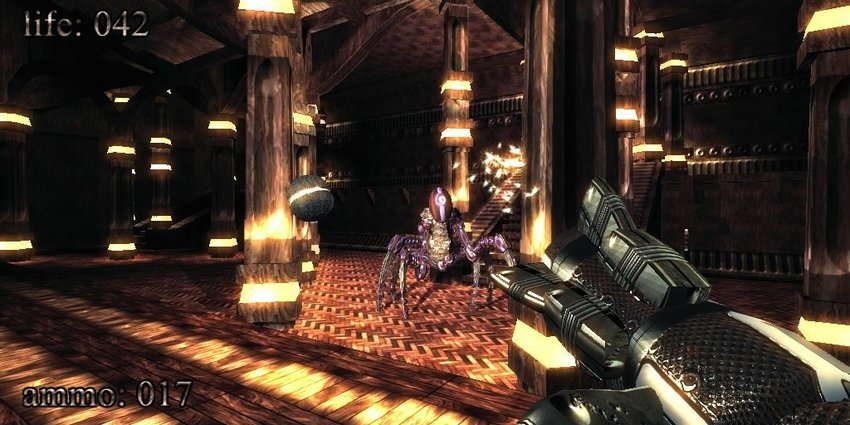
\includegraphics[width=0.75\textwidth]{Images/kkrieger.png}
	\caption{The game .kkrieger, which uses procedural generation to design maps while keeping the game at a 96 kilobyte file size.\cite{pcgvirtualworld}}
	\label{fig:kkrieger}
\end{figure}

Other games that use procedural generation in its levels include Elite (originally published in 1984), Elite: Dangerous (2012), Minecraft (2009), No Man's Sky (2012) and Spelunky (2013). \href{https://youtu.be/Uqk5Zf0tw3o}{The latter game's use of procedural generation has notably been covered by video games journalist Mark Brown in a YouTube video.}\cite{spelunkyvid}

\begin{figure}[H]
	\centering
	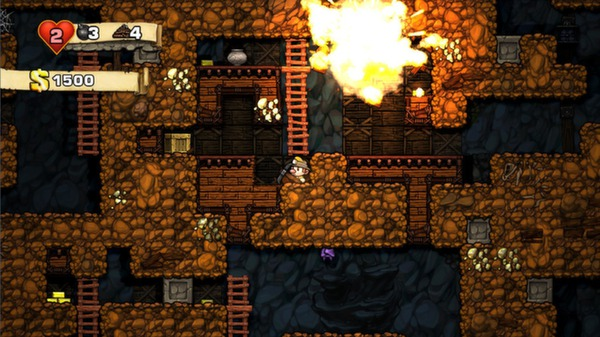
\includegraphics[width=0.7\textwidth]{Images/spelunky.jpg}
	\caption{\href{https://spelunkyworld.com/}{The roguelike game Spelunky}, which uses procedural generation to build intricate levels for the player character to explore.\\Source: \link{https://store.steampowered.com/app/239350/Spelunky/}}
	\label{fig:spelunky}
\end{figure}

In many cases, these games end up having a \textbf{large} number of different environments that each game could generate for its players. However, by procedurally generating them upon the \textit{loading} of the game level, in lieu of loading a layout from disk, they can save a lot of space (albeit with a considerable need for processing power, depending on the game's and algorithms' performance), as seen in Figure \ref{fig:kkrieger}.

Using one or some different procedural generation algorithms, such as the use of Perlin, Simplex or other noise, Voronoï disks and also poisson disk generation, among others, games can load a seed to randomly generate a level every time it is played, meaning no two playthroughs of a game with procedurally generated content are ever the same.

\section{Justifying My Choice of Engine: Godot}

While a myriad of resources exist for procedurally generated game contents exist for Unity and Unreal, I want to implement them in Godot, for several reasons:

\begin{itemize}
	\item It's the engine I have the most experience with, having already developed 2 published web games with it.
	\item It's not got as many resources on procedural generation compared to Unity, Unreal and some other popular game engines, particularly on the side of academic research (that is, there aren't as many papers on procedural generation that pertain to Godot as they do to Unity, Unreal and other engines).
	\begin{itemize}
		\item However, it is still very powerful and feature-rich (it has its own Open Simplex noise class, for example) and I'm sure I can make procedural generation algorithms work on it.
	\end{itemize}
	\item Compared to Unity and Unreal, Godot is a very light engine with a feature-rich editor, clocking in at under 100MB, with editors for Windows, macOS, Linux and even the web browser. 
\end{itemize}

By the end of my allotted time, I plan to have implemented several procedurally generated environments in small Godot games, using a myriad of methods (such as Voronoï cells and poisson disk generation) in a myriad of contexts (anything from platformers to first-person games). With these games, I plan for the final report to be the centrepiece of my project, with it containing my research on how each environment was implemented, as well as my findings on the algorithms themselves and how they work.

This is somewhere between a research-oriented project and an implementation-oriented project, as while the produced software artifacts provide valid proof of my understanding of some commonly used procedural generation algorithms and how to implement them in Godot, it is also about how I understand their workings. Nonetheless, the implementations provide the weight behind my project's motivations and are the main focus of this dissertation. They will prove that Godot is just as adept at procedural content generation as the other major players in the game engine space, and I will have gained a wealth of knowledge on PCG in the process.

\subsection{Note on Differing Versions of Godot}

Godot currently is at version 4, which finally received a stable release in 4\textsuperscript{th} March after years of development, but concurrently there is also Godot 3, the previous stable version which is now a \textbf{L}ong-\textbf{T}erm \textbf{S}upport release. The latter version of Godot contains several new features and breaking changes, so any project made in Godot 3 won't readily be compatible with Godot 4 (and vice-versa) without making the necessary changes and conversions. I have access to both versions of Godot and, for all the Godot projects I made and used in this project, I have used Godot 4. Any references to other Godot 3 projects will be clearly denoted as such.

\section{Justifying My Choice of Scenario: A 2D tile-map RPG-style roaming game}

The scenario of my choosing involves a monochrome tile-map created by Kenney.nl in a 2D RPG setting, in which the player character is a hollow ``Golem" that is trying to search for and obtain a ring among a large 72x40 village, filled with trees, buildings and emptiness. The player can ``chow down" trees by simply going to the cells where trees are and making them disappear. However, the player \textit{will} stop at and collide with any buildings in the tile map. When the player collects the ring, they win the game and are able to either close the window or generate a new village to try and collect \textit{another} ring.

The size of the tile map is determined by taking the window size, 1152x640 in \textbf{all} implementations, and then dividing it with the cell size, 16x16 in \textbf{all} implementations (again), hence returning a 72x40 tile map size. Using a large tile map like this, with 2880 available cells in total, allows for easy stress-testing of the algorithms, making them generate level layouts that are sufficiently large enough to produce a quantifiable performance result and time that can be easily compared across implementations, such that we can easily measure how one performs over the other. The use of a tile map \textit{this} large with PCG algorithms also makes sense from a game developer's perspective as designing level layouts this large by hand, with such a small cell size as well (inherited from the size of the tile map assets), would add additional time and labour costs to them. 

The use of a tiled role-playing game scenario, adapted to already-existing procedural generation algorithms, is relatively unusual in the context of procedural generation. However, it \textit{will} allow me to go a degree beyond the scope of what is usually done for procedural content generation in games, which is usually seen in 2D and 3D roguelikes and platformers, as well as some other world-building games such as Minecraft and Terrraria, while also producing code that is relatively easy to process through and understand. The ability for the player character to consume trees and remove them from the level layout by moving into them allows that player to easily move around in what would otherwise be very crowded level layouts that would have been near-impossible to traverse. The addition of said player character, as well as the end goal of obtaining a randomly-placed ring within the given level, adds weight to the algorithms' practical use in games made with Godot, and not just for show or solely as demonstrations. 

\section{Justifying My Choice of Algorithms for the Above Scenario}

For this project, I intend to use the following procedural content generation algorithms within my scenario:

\begin{enumerate}
    \item Lindenmayer Systems (or L-Systems)
    \item Perlin and Simplex Noise
    \item Poisson Disk Sampling/Distribution
    \item Voronoï Cells/Diagrams
\end{enumerate}

Using an L-System for generating a level layout is relatively uncommon, compared to its use in generating structures such as trees and buildings. However, I plan to integrate a deterministic context-free L-System (or a ``D0L-System") into an implementation of my scenario so I can compare it performance-wise to the other algorithms, and see how the repeated patterns generated from L-System grammars affect comparisons to the other implementations' level layouts. 

Perlin and Simplex Noise are far more commonly used for level layouts, so I created an implementation of my scenario with one to see how it compares with the others, speed-wise and layout-wise, and see if it really is the best for my chosen scenario.

Poisson Disk Sampling is usually used for item placement in planes, even with grids, so using a grid-like implementation, I will compare how it works with in a tile map and what differences arise between its use there and in its usual uses.

Though efforts were made to make level layouts as similar as possible across implementations, there are noticeable differences between the level layouts generated by L-Systems, Simplex noise and Poisson disk samples, and I touch on those when discussing those implementations in the relevant sections of my report.

In my research and implementation of Voronoï Cells I realised the level layouts it generated for my scenario were wholly unique, when compared with the other algorithm implementations, so much so that I had to re-shape my scenario and game mechanics to make both the scenario and levels generated fit with each other. Nonetheless, I believe this will serve as a unique comparison to the other algorithms and will serve as additional knowledge of procedural generation algorithms as well as more work towards understanding how to make them work in Godot games (as proven by my implementations).
\chapter{Report Body}
%The central part of the report usually consists of three or four chapters detailing the technical work undertaken during the project. {\bf{\textcolor{red}{The structure of these chapters is highly project dependent}}}. They can reflect the chronological development of the project, e.g. design, implementation, experimentation, optimisation, evaluation, etc (although this is not always the best approach). However you choose to structure this part of the report, you should make it clear how you arrived at your chosen approach in preference to other alternatives. In terms of the software that you produce, you should describe and justify the design of your programs at some high level, e.g. using OMT, Z, VDL, etc., and you should document any interesting problems with, or features of, your implementation. Integration and testing are also important to discuss in some cases. You may include fragments of your source code in the main body of the report to illustrate points; the full source code is included in an appendix to your written report.

In this chapter, I will explain how each of my chosen algorithms work, and how I went around implementing them as a surface-level explanation. I will then briefly compare what challenges I faced for each of my implementations, and how they compare, both performance-wise and with regards to the kinds of layouts they produce, again as surface-level explanations. I go into greater detail on my implementations in the Implementation section, how the level layouts generated in each algorithm compare with each other in the Design \& Specification section, and how each implementation compares overall (and also performance wise) in the Evaluation section. For this project, I chose to use the following 4 algorithms.

\begin{enumerate}
    \item Lindenmayer Systems (or L-Systems)
    \item Perlin/Simplex Noise
    \item Poisson Disk Sampling
    \item Voronoï Cells
\end{enumerate}

\section{Algorithms}

In this section, I will explain how each of the algorithms I implemented work, then I will go into small detail as to how I implemented them. I go into further detail in the ``Implementation" section of this report.

\subsection{Lindenmayer Systems}

Hungarian academic Aristid Lindenmayer devised a mathematical model for the reproduction of fungi in 1967.\cite{LINDENMAYER1968300} His model involved a string of symbols, each unique symbol denoting a specific action and/or branch. Essentially, running that initial string, called the \emph{axiom}, through a set of rules (called a \emph{grammar}) gives us an ever-expanding string that is then taken as instructions to draw something from. Lindenmayer Systems, or L-Systems, have since been used in several scenarios beyond its initial purpose of modelling fungi, from trees to fractals. In video games, they are frequently used to aid in the creation of foliage in several environments, as well as buildings and, here, level layouts.

\subsubsection{A Basic 0L-System}

The most basic form of L-System is a \emph{0L}-System, 0 in this case referring to the fact that the grammar is \emph{context-free}.

For this example\cite{lsyspaulbourke}, consider an alphabet $V$, which consists of the following symbols:

\newcommand{\F}{\mbox{F}}

$$ \F, +, - $$

where $\F$ means ``to go forward", and $+$ and $-$ denote turning right or left (respectively) a set number of degrees $\o$.

Take an axiom $\omega$, for example:

$$ \F+\F+\F+\F $$

And a set of rules $P$ which, in this case, is of size 1:

$$ \F \rightarrow \F+\F-\F-\F\F+\F+\F-\F $$

We can represent this \emph{parametric} L-system in the following form:\cite{enwiki:1124510226}

$$ G = (V, \omega, P) $$

To implement $G$ in Godot, we can take each rule and replace each string in accordance to our one rule, using the replace method, like so:

\begin{figure}[H]
    \centering
    \begin{lstlisting}
string = string.replace(rule["from"], rule["to"]) #Here the rules were stored in dictionaries.
    \end{lstlisting}
    \caption{A line of code that demonstrates directly replacing characters in a string according to our L-System grammar's rules.}
    \label{fig:lsys-snippet-1}
\end{figure}

The first 3 iterations of this operation are shown here:

\begin{figure}[H]
	\centering
	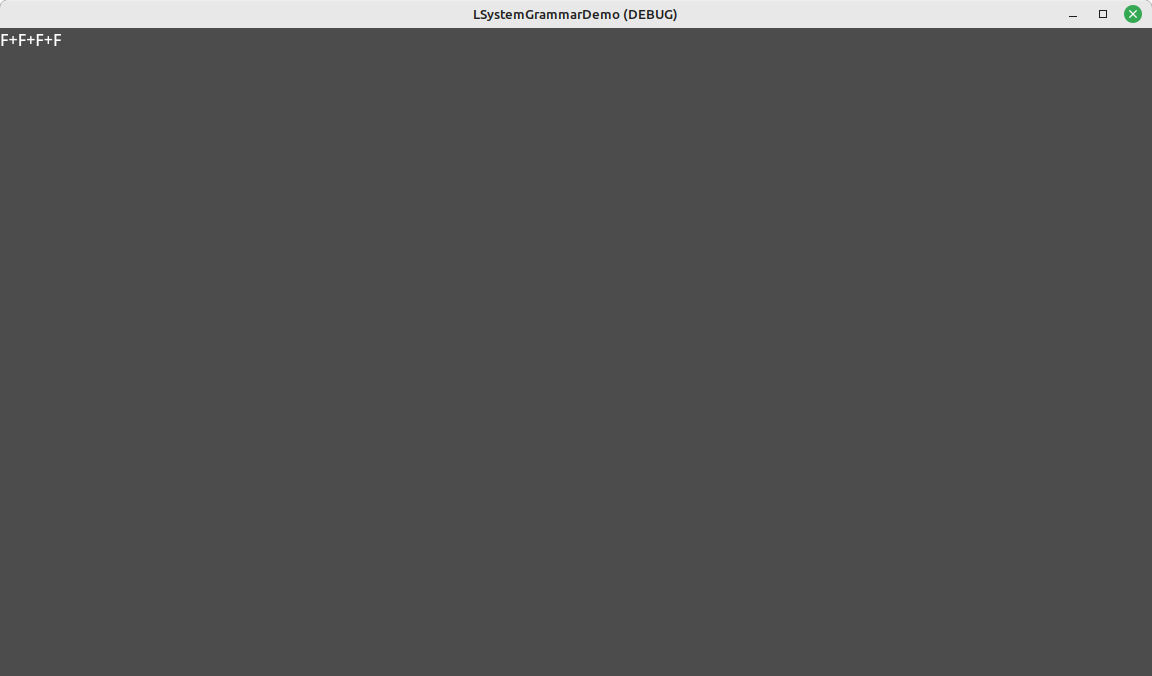
\includegraphics[width=0.5\textwidth]{Images/initial-l-system-iteration-0.png}
	\caption{The axiom of the aforementioned simple L-System with just one rule. String size: 8.\\Source: Own work.}
	\label{fig:lsysiter0}
\end{figure}

\begin{figure}[H]
	\centering
	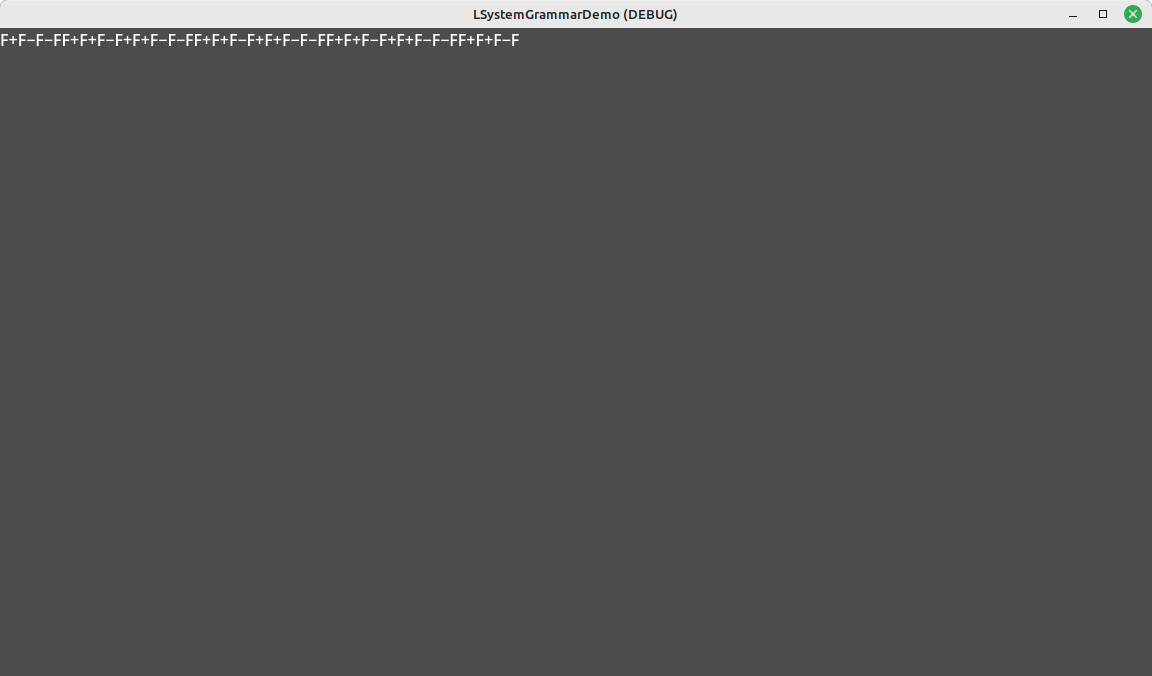
\includegraphics[width=0.5\textwidth]{Images/initial-l-system-iteration-1.png}
	\caption{The first iteration of the aforementioned simple L-System with just one rule. String size: 59.\\Source: Own work.}
	\label{fig:lsysiter1}
\end{figure}

\begin{figure}[H]
	\centering
	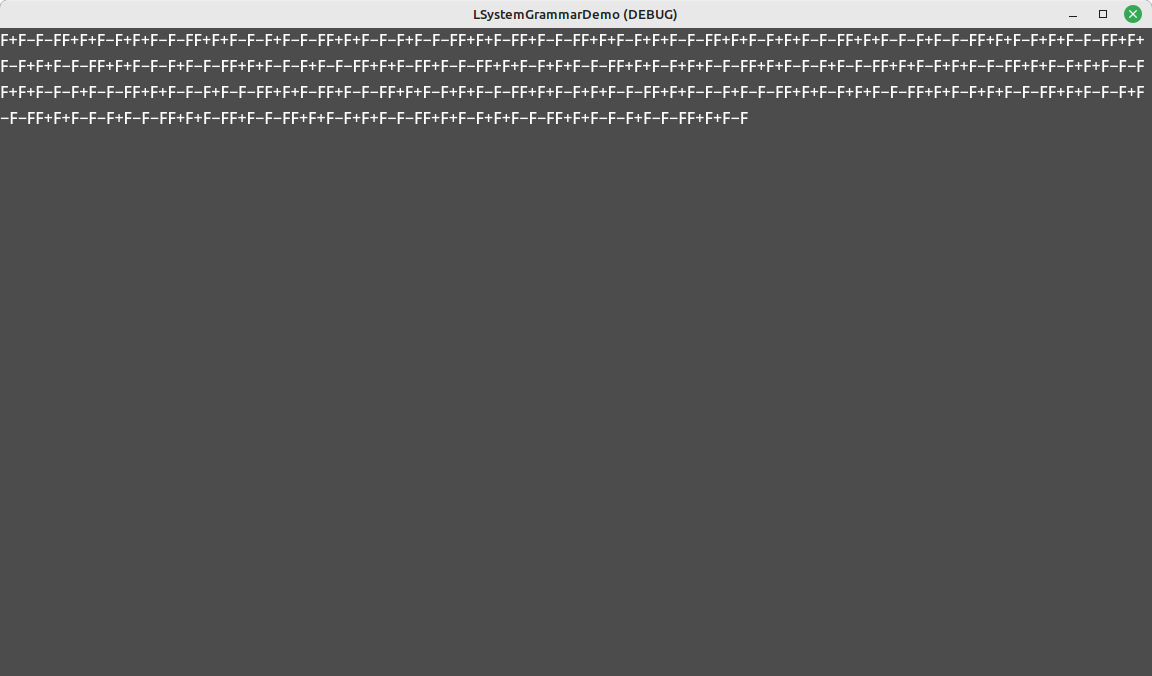
\includegraphics[width=0.5\textwidth]{Images/initial-l-system-iteration-2.png}
	\caption{The second iteration of the aforementioned simple L-System with just one rule. String size: 475.\\Source: Own work.}
	\label{fig:lsysiter2}
\end{figure}

\begin{figure}[H]
	\centering
	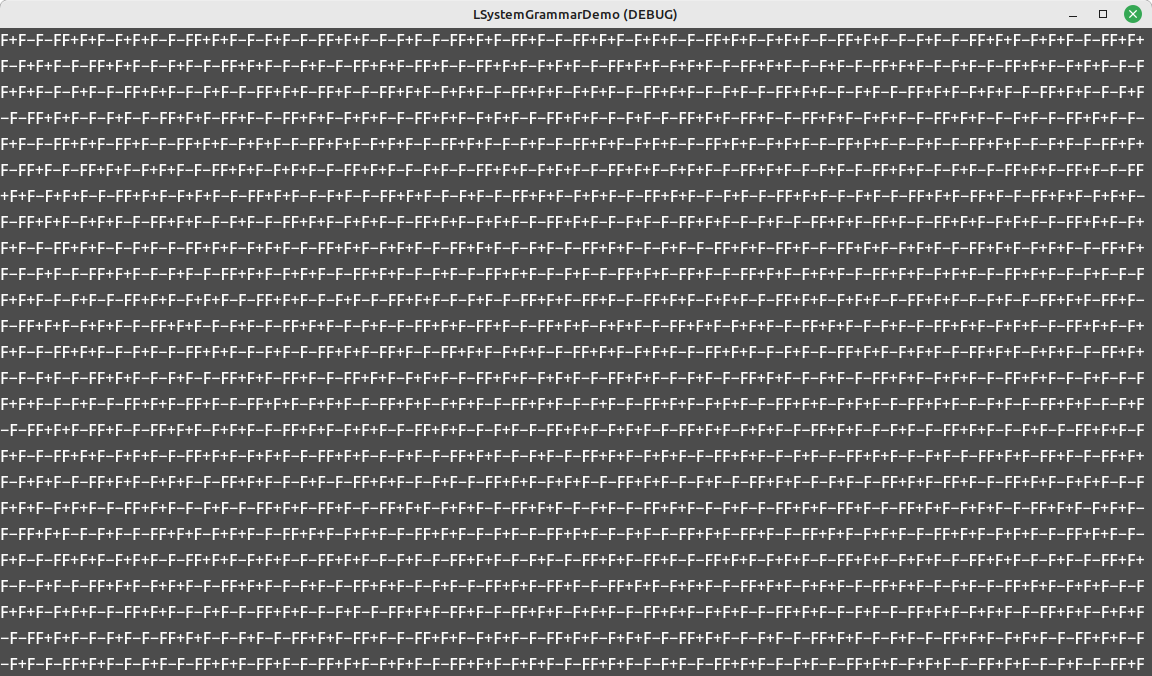
\includegraphics[width=0.5\textwidth]{Images/initial-l-system-iteration-3.png}
	\caption{The third iteration of the aforementioned simple L-System with just one rule. String size: 3803. The string is too large to show in the window, as you can see here.\\Source: Own work.}
	\label{fig:lsysiter3}
\end{figure}

The resulting string can be used to draw a lattice.\cite{lsyspaulbourke} Examples of the above grammar in action are below.

\begin{figure}[H]
    \centering
    
\includegraphics[height=0.25\textheight]{Images/lsys03.png}
    \caption{A lattice generated with the example grammar on a custom-written Classic Mac OS application specifically written for working with L-Systems.\cite{lsyspaulbourke}}
    \label{fig:lattice1}
\end{figure}

\begin{figure}[H]
    \centering
    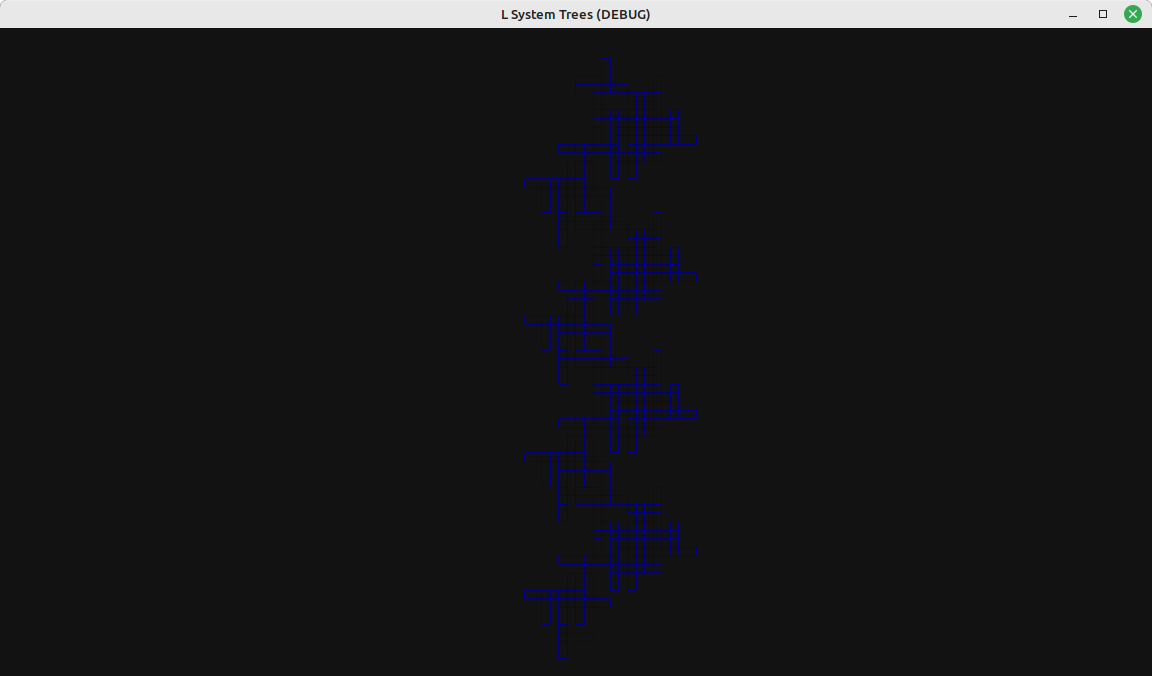
\includegraphics[width=0.75\textwidth]{Images/gd4lattice.png}
    \caption{A lattice generated with the example grammar on a Godot project for drawing from L-Systems. Source: Initial project written by YouTuber Codat\cite{codatGD3LSystemYT}\cite{codatGD3LSystemGH}, and converted to Godot 4 (with the addition of the lattice grammar) by me.\cite{codatGD4LSystemGH}}
    \label{fig:lattice2}
\end{figure}

\subsubsection{A More Complex D0L-System With More Than One Rule}

For handling more than one rule, we can instead use a new string buffer variable where, for each character in our string, we can attain a new string and append it to our string buffer. The resulting string is then returned and interpreted. This can be represented in Godot as demonstrated in Figure \ref{fig:lsys-snippet-2}, which uses two functions to perform string replacement. The first function \verb|get_new_replacement| performs the character replacement according to the L-System's grammar rules, while the second function \verb|replace_string| uses a string builder variable to allow for replacement of characters without directly affecting the original string and causing unwanted side effects.

\begin{figure}[H]
    \centering
    \begin{lstlisting}
func get_new_replacement(character: String) -> String:
	for rule in rules:
		if rule["from"] == character:
			return rule["to"]
	return character

func replace_string(string: String) -> String:
	var new_string = ""
	for character in string:
		new_string += get_new_replacement(character)
	return new_string
    \end{lstlisting}
    \caption{Two GDScript functions for replacing characters in an L-System grammar with more than one rule.}
    \label{fig:lsys-snippet-2}
\end{figure}

This can \textit{then} be used to handle more complex grammars that can handle more than one rule in which characters in strings are replaced by other strings of variable length, as before.

The grammar in the following example represents a D0L-System\cite{lsystemintro}, a \textbf{deterministic} L-System using a context-free grammar; the grammar in the first example was \textit{also} deterministic.

\newcommand{\A}{\mbox{a}}
\newcommand{\B}{\mbox{b}}

For this example, consider a new grammar $G$ with the alphabet $V$, where $\A$ and $\B$ are the only symbols. We start with the following axiom $\omega$, which is just $\A$. We now have a set of rules $P$ which is, this time, of size \textit{2}:

$$ \A \rightarrow \A\B $$
$$ \B \rightarrow \A $$

The first few steps of the resulting derivation can be modelled like so:

\begin{figure}[H]
    \centering
    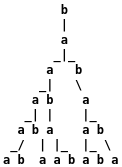
\includegraphics[scale=0.5]{Images/derivationtree.png}
    \caption{The first few steps of a derivation of our example grammar.\cite{lsystemintro}}
    \label{fig:derivationtree}
\end{figure}

\subsection{Perlin/Simplex Noise}

Traditionally, white noise images, and most other noise types, place noise pixels completely randomly, without each pixel considering the values of its neighbours\cite{gd3perlinnoise}, as you can see in Figure \ref{fig:whitenoisepic}.

However, there exists several types of \textbf{value} and \textbf{gradient} noise that \textit{do} take surrounding pixel values into consideration, and will therefore serve more use in building levels in our games.

Value noise simply takes a lattice of points with random values and then interpolates those points based on their surrounding values. This \textit{can} be used as a procedural texture. However, due to the simple nature of the algorithm, it's possible that the difference between several values in a region is minimal, while in other regions the values may differ immensely, resulting in a noise image that is not very smooth.

Gradient noise, on the other hand, takes point lattices and instead calculates the interpolation between tangents.\cite{perlinvalue} Since both tangents between a curve must be collinear\cite{perlinvalue}, the flat and bumpy curves produced by value noise's interpolation calculations are now much less likely to be returned, as seen in Figure \ref{fig:valueperlincomparison}.\cite{perlinvalue} This results in noise images of higher and more appealing visual quality as, to quote a response from Stack Exchange by Hernan J. González\cite{gradientvalue}, ``it cuts low frequencies and emphasizes frequencies around and above the grid spacing."

\begin{figure}[H]
    \centering
    
\includegraphics[width=0.75\textwidth]{Images/whitenoisepic.png}
    \caption{A white noise picture generated with Robson's white noise image generator.\cite{whitenoisepicgen}\\Settings: 640 squares horizontally, 480 squares vertically, size of squares 1, colours greyscale, bias none.}
    \label{fig:whitenoisepic}
\end{figure}

\begin{figure}[H]
    \centering
    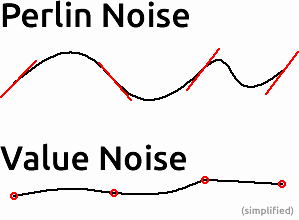
\includegraphics[width=0.75\textwidth]{Images/valueperlincomparison.png}
    \caption{A comparison between the kinds of curves produced by Value noise interpolation and Perlin (and other Gradient) noise interpolation.\cite{perlinvalue}}
    \label{fig:valueperlincomparison}
\end{figure}

Two particularly well-known Gradient noise algorithms that are commonly used for procedurally generating levels are the already mentioned Perlin Noise and Simplex Noise, both designed by American Computer Science professor Kenneth H. Perlin, with the former being an improvement on the former. Perlin Noise also takes a lattice of randomly assigned gradients, but the algorithm interpolates the dot products of those points instead of just their neighouring values.\cite{fastnoiselitedocs} Simplex noise, meanwhile, tries to reduce the grid artifacts caused by the original algorithm, and has the added benefit of scaling better to larger dimensions.\cite{pcgwikisimplex} Perlin filed a patent on his work in 2002 that was granted in 2005\cite{perlinpatent}, which prompted the creation of the OpenSimplex noise algorithm\cite{enwiki:1102898483} for free use; the patent has since expired in 2022, allowing free use to both Perlin and the original Simplex noise.\cite{perlinpatent}

Godot 3 previously featured an OpenSimplexNoise class for generating noise textures, which used the OpenSimplex algorithm. This algorithm 

\subsection{Poisson Disk Sampling}

Poisson disk distributions are an easy way to randomly scatter objects across a field. It's commonly used for tree placement and placement of other random objects. Points are placed over a plane, with a single point placed randomly and subsequent points calculated such that a single point has no other point lying within a given radius of said point. Different implementations of Poisson disk distributions or samples can accommodate multiple radii for points in a plane, and some implementations produce \textit{maximal} samples- that is, a set of samples that fully cover the given plane, while still adhering to the principle that no single point has other points lying within its radius\cite{10.1145/1964921.1964944} (the implementation I made for this project does \textbf{not} guarantee maximality, however).

The following are some examples of Poisson disk distribution in action:

\begin{figure}[H]
    \centering
    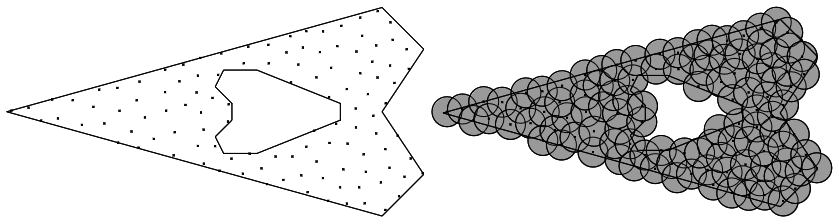
\includegraphics[width=\textwidth]{Images/maximalpoissonsample.png}
    \caption{A diagram of a maximal Poisson disk distribution done on a concave plane, with the right side denoting maximality through the grey disks overlapping but not any points overlapping.\cite{10.1145/1964921.1964944}}
    \label{fig:maximalpoisson}
\end{figure}

\begin{figure}[H]
    \centering
    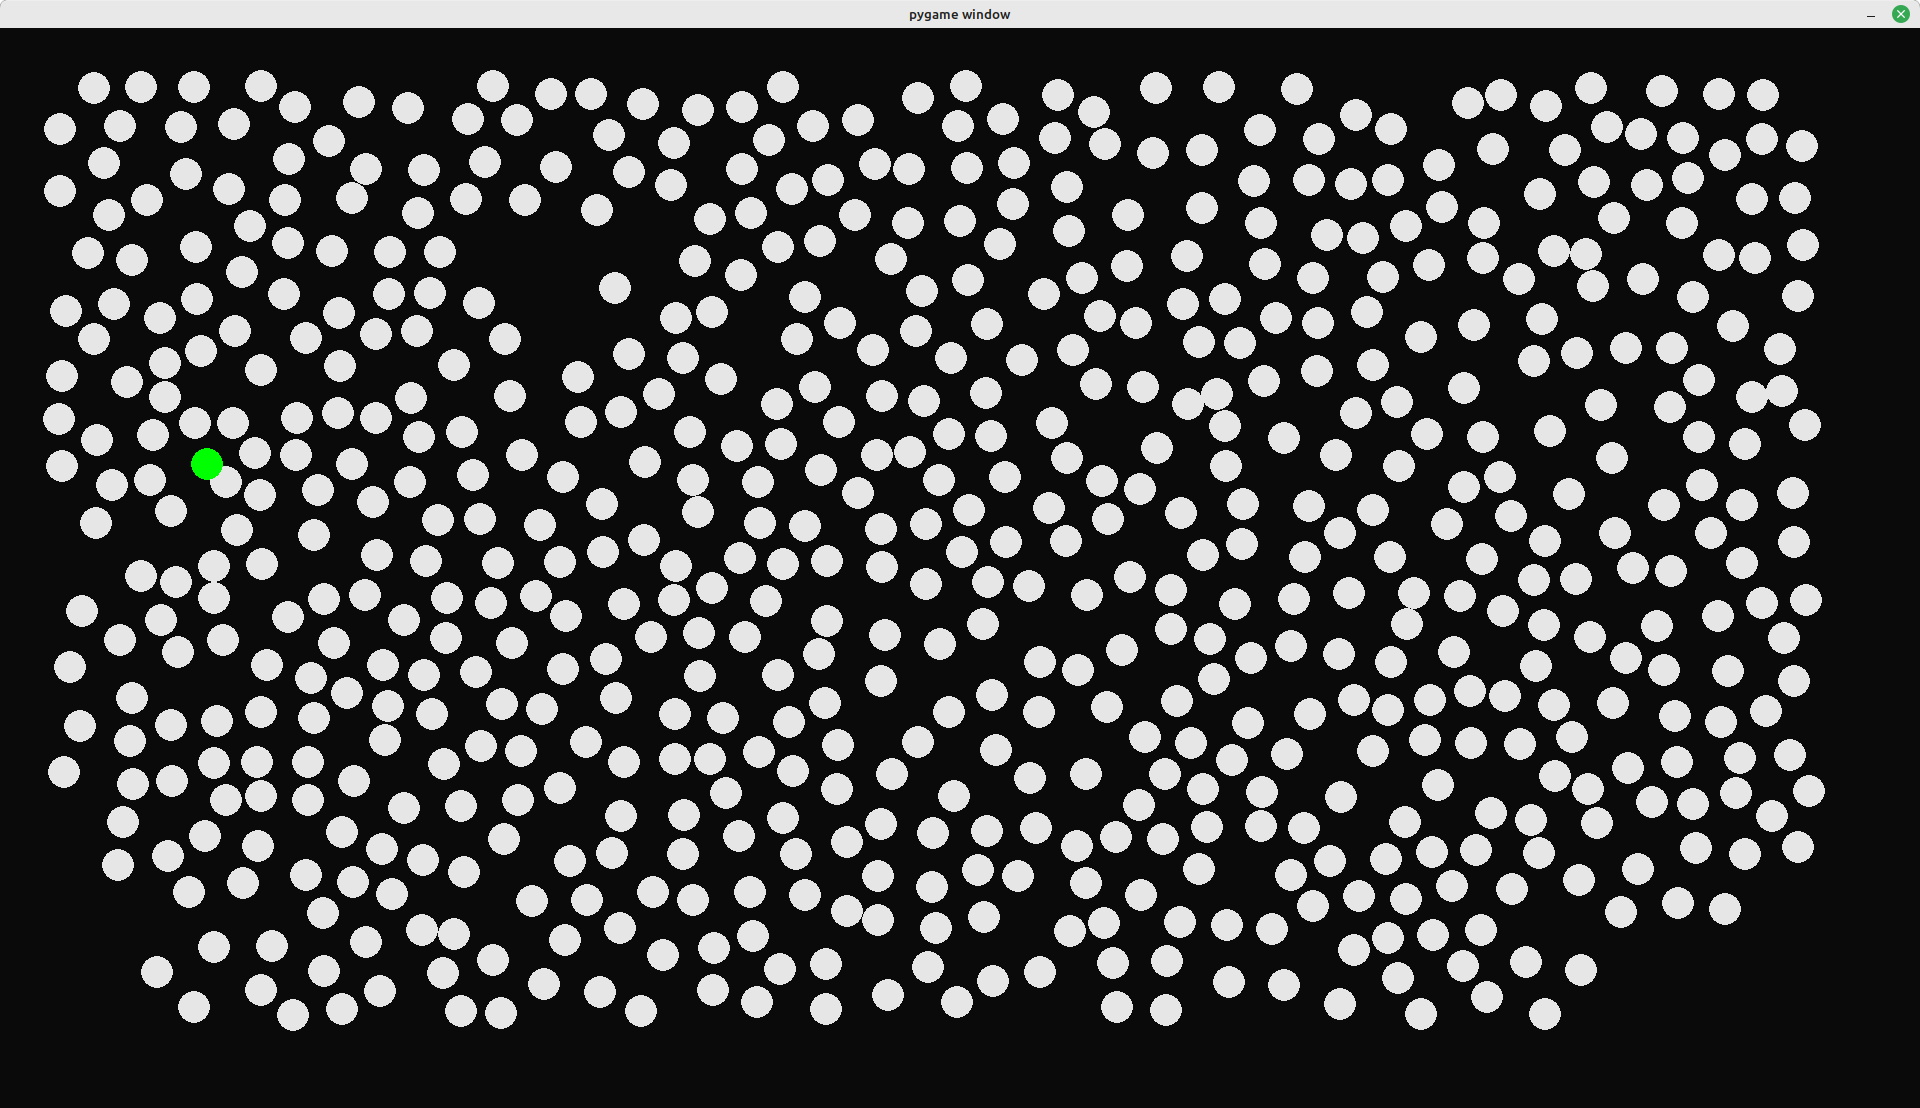
\includegraphics[width=\textwidth]{Images/pygamepoissonsample.png}
    \caption{An implementation of Poisson disk sampling made in Pygame.\cite{pygamepoissondisksampling} The screenshot was taken \textit{after} all of the samples were taken.}
    \label{fig:pygamepoisson}
\end{figure}

\subsection{Voronoï Cells}

Named after the Ukranian mathematician Georgy Voronoy, Voronoï cells work by taking a map of points, and randomly selecting a group of points. Within that selected group, cells are formed by calculating, in each point of the grid, the closest of the selected points to it. That is, each cell represents the group of points that are the closest to that random point (including that point in the group as well). The final arrangement of cells represents a Voronoï Diagram or Voronoï Tesselation.

Distances between points can be calculated with either the Euclidean distance:

$$ d_{E}(p, q) = \sqrt{(q_x - p_x)^2 + (q_y - p_y)^2} $$

or the Manhattan distance:

$$ d_{M}(p, q) = |q_x - p_x| + |q_y - p_y| $$

With the Euclidean distance producing a more ``triangulated" tesselation than the Manhattan distance, with straighter diagonals and cells shaped like irregular polygons, the geometry of which is more "blocky" and resembles taxicabs (hence its alternate name "Taxicab Geometry"). A visual comparison of the kinds of cells generated with either distance calculation is shown in Figure \ref{fig:voronoicomparison}.

\begin{figure}[H]
    \centering
    \includegraphics{Images/Voronoitessellations.jpg}
    \caption{A visual comparison of the kinds of Voronoï cells generated with the Euclidean and Manhattan distance.\cite{reffortesselations}}
    \label{fig:voronoicomparison}
\end{figure}

\section{Implementations}

Here I will describe, at surface level, the methods I went about implementing the above algorithms and what references I used.

\subsection{Commonalities Between Implementations}

To implement the same scenario, aforementioned in the background of this report, across all 4 algorithm implementations, I had to include some of the same code and functions, as well as the same tile set shown in Figure \ref{fig:kenneyset}.

From this tileset, which contains 1078 tiles, my code uses 27 building tiles, 13 tiles for trees and other fauna, 1 tile for the player character and one of 4 tiles for the ring. The relevant coordinates of the tiles for buildings, trees and the ring are each stored in constant arrays in the script, while the player tile's coordinates are just stored in a local constant (not an array, since there is no need for one).

To handle player placement and subsequent movement, I have several functions. Godot's built in \verb|physics_process| function handles events that happen in real-time, and is commonly used, like in this context, for player movement. In it, I first store the current player's cell, \verb|player_movement_cell|, in \verb|previous_cell|, then I initialise a \verb|direction| based on which input movement was pressed (\verb|Vector2i.LEFT| when \verb|"ui_left"| was pressed, and so on). Then I add the player's current cell with the direction to calculate the potential \verb|new_movement_cell|. If this cell is within the bounds of the enviroment, as well as either a tree or empty space (or the ring), it moves there, and the previous cell gets erased. If the player ends up moving into the cell where the ring is, the player wins the game, and all movement is paused while a winner's dialog popup shows up. The player moves \textbf{very} quickly in our games, and I have yet to figure out how to slow down this movement while also not making movement so slow that the games drags; the player will not want to have to continually press down an arrow key to move to 1 cell in a map of 2880 cells. Since the performance of the algorithms are more important in this project, however, I decided to leave the very fast player movement as is.

I have written \verb|place_player| and \verb|place_ring| functions that handle the random generation of the player's and ring's initial starting positions. Both use the \verb|_get_random_placement_cell| helper function to retrieve a new cell, and both use a while loop to make sure the randomly generated cell isn't already occupied. In both functions the placement cells are assign and calculated \textbf{before} the while loop, so that their placements do not default to just (0, 0) in the beginning.

\begin{figure}[H]
    \centering
    
\includegraphics[width=\textwidth]{Images/monochrome_packed.png}
    \caption{The tileset used for all 4 implementations of my scenario with PCG algorithms.\cite{kenneyassetsused} Of all the 1078 tiles, of size 16x16, in this tileset, only 45 of them get referenced in my code.}
    \label{fig:kenneyset}
\end{figure}

Across all implementations, there are two local variables, \verb|x_tile_range| and \verb|y_tile_range|. Both of these calculate the dimensions of our tile map by taking the display window's respective x and y dimensions from the project's settings (1152x640) and divides them by the respective x and y dimensions of the cell size (16x16). \verb|x_tile_range| should resolve to 72 upon runtime, and \verb|y_tile_range| should equal 40, giving us our 72x40 tile map that gives us a total of 2880 cells to work with in our games.

Finally, there are two dialog popups added to each scene tree, one for describing the game's story (\verb|AcceptDialog|, of type \verb|AcceptDialog|) and another for when the game ends after the player has collected the ring (\verb|WinDialog|, of type \verb|ConfirmationDialog|). For \verb|AcceptDialog| the \verb|confirmed| and \verb|canceled| signals are both connected to the function \verb|_on_AcceptDialog_closed|, which hides the popup and unpauses the game. For \verb|WinDialog|, on the other hand, \verb|confirmed| is connected to \verb|_on_WinDialog_confirmed| and \verb|canceled| is connected to \verb|_on_WinDialog_canceled|. \verb|_on_WinDialog_confirmed| is meant to generate a new level layout, while \verb|_on_WinDialog_canceled| is meant to close the game, both when the cancel button (labelled "Get Me Out of Here") is clicked and when the cross on the top-right corner of the popup is clicked. However, as of now, only the top-right corner of both popups does what it is supposed to; clicking any of the other buttons from both popups, for some reason, does nothing at the moment, and I \textit{did} make sure, in my code, that the signals were properly connected. However, the games themselves still run as they are supposed to, and the integration of the algorithms into the levels in the games are more important here, so since \textit{they} still work, I decided to leave the popups, their behaviour and their code as they were. \textit{If} they are engine issues, regarding the buttons, they may hopefully get fixed in future versions of Godot.

\subsection{Lindenmayer System}

The implementation of an L-System was very simple. I took inspiration from a YouTube video on implementing an L-System for drawing line graphics in Godot by Codat.\cite{codatGD3LSystemYT} In the code from the Godot 3 project he made in that video\cite{codatGD3LSystemGH}\cite{codatGD3LSystemYT}, he created a custom ``Rule" class in GDScript, with which he defined new rules. I forked his project, converted it to Godot 4 and used it to create the lattice graphics in Figure \ref{fig:lattice2}.\cite{codatGD4LSystemGH} I did this mainly as a reference for my implementation of L-Systems in the game itself.

With the implementation in my \emph{game}, I adapted the \verb|get_new_character| method in that L-System to work with the dictionary I originally implemented my L-System in. The new \verb|get_new_replacement| method in my implementation allows for there to be more than one grammar rule while the L-System still performs as it should. My original L-System iterated through the original string \textit{directly}, which produced unintended consequences in grammars with multiple rules, as seen here when trying to implement the D0L-System I mentioned earlier\cite{lsystemintro}:

$$ b \rightarrow a \rightarrow aa \rightarrow aaa \rightarrow aaaa \rightarrow aaaaa \ldots $$

By using an empty string buffer and inserting rule replacements there instead, my implementation is now able to perform substitutions accordingly; the correct computation of the D0L-System is denoted in Figure \ref{fig:derivationtree} and repeated below:

$$ b \rightarrow a \rightarrow ab \rightarrow aba \rightarrow abaab \rightarrow abaababa \ldots $$

With the L-System string parsing algorithm in place, the next step was to paint the cells of each tile. With this, I iterated through every cell of the tilemap using a nested for-loop. With the parsed string, I then accessed the character of the string at an incremented index using an iterator variable I defined before the for-loops. The string consists of three different characters repeated multiple times, ``O", ``W" and ``B". For each string index, if the character is ``W", paint a tree, if it is ``B", paint a building, and if it is an ``O", leave the cell blank and paint nothing. The player and ring then get placed afterwards.

Even for a large-sized tile map with 2880 cells, a constant L-System $G$, with the symbols O, W and B and the following grammar

$$ \mbox{O} \rightarrow \mbox{O}\mbox{W}\mbox{O} $$
$$ \mbox{W} \rightarrow \mbox{W}\mbox{B} $$
$$ \mbox{B} \rightarrow \mbox{B}\mbox{W}\mbox{O} $$

can parse the axiom OWB, paint tile map tiles with the resulting string \textbf{and} place the player and ring in just 19 milliseconds on average. This was the default grammar used by the L-System in the game. I also included 3 more grammars, one that generated more buildings (and impossible level layouts), another that generated more trees and another that generated more empty space. These can be easily selected with the \verb|ruleset| export variable in the Godot editor. Further variance can be added with the addition of a randomly generated axiom, capped at a maximum height or smaller (minimum 1). If said option is enabled in the Godot editor, the default value in the export variable for setting this cap is 10, and since it is an export variable, it too can be adjusted in the editor as the developer sees fit.

\subsection{Perlin/Simplex Noise}

The Simplex Noise implementation works with Godot's built-in Noise library. Within a Sprite2D node's Texture attribute, I set a new ``NoiseTexture2D" field inside of it. In its ``Noise" attribute I created a new ``FastNoiseLite" scene, which generates a noise texture for us to use. The seed can be set in the sprite's script file.

As with my other implementations, there are two separate arrays, one for trees and another for buildings. For each cell in the TileMap, I then took the noise pixel from the generated texture at that exact point (scaling with the cell size accordingly), using the \verb|get_noise_2d| method built-in with Godot, and then, depending on the value retrieved, decided, firstly, whether or not to place a plant/tree tile there and, secondly, whether or not to place a building tile there. As a result, not every cell in the TileMap has tiles on it. On any one of those empty cells, the Player tile will then get placed.

For the generation of the noise itself, I \textit{could've} added a \verb|Sprite2D| node to the scene tree, the root of which was my \verb|TileMap|, and gave it a \verb|NoiseTexture2D| texture and set its \verb|noise| property to a newly-created \verb|FastNoiseLite| instance, the latter of which contains the actual noise data. In the early stages of this implementation's development, that's what I did, and I created a script that solely set the seed of the \verb|FastNoiseLite| resource to a random integer (using the \verb|randi| method). However, for a more authentic result, and to forgo the need of an additional node and noise texture that will not even be visible in the final product, I decided to create the noise for this algorithm implementation entirely programmatically. I stored the \verb|FastNoiseLite| instance in its own class variable \verb|noise|, and instantiated it with the \verb|set_noise| method when starting the game (the \verb|_ready| function automatically runs when the game starts).

Initially having done the noise integration with a sprite node and noise texture allowed me to experiment with some of the \verb|FastNoiseLite| class's properties before finally resorting to programmatic noise creation. An instance of this class, by default, uses the ``Simplex Smooth" noise algorithm, a version of the Simplex algorithm that produces higher quality noise images at the expense of slower speed.\cite{fastnoiselitedocs} We can also use just ``Simplex" noise for higher speed, as well as the original ``Perlin" noise algorithm.\cite{fastnoiselitedocs} Godot also allows us to use two kinds of Value noise, as well as a ``Cellular" type that combines algorithms like Worley Noise and Voronoï diagrams to create "regions of the same value."\cite{fastnoiselitedocs} I had problems with the ``Cellular" noise type when experimenting with it, for reasons I will get into later, but the other noise types I made readily accessible in an ``export" variable in my script (that is, a variable that can be easily accessed in the Godot editor when the TileMap node is clicked on) when I removed the sprite node and decided to programmatically make the noise. When the \verb|set_noise| function is called, the noise type is assigned through the \verb|_get_noise_type| function, which returns an integer value depending on the type of noise selected, and the returned result is cast to \verb|FastNoiseLite|'s \verb|NoiseType| enumeration\cite{fastnoiselitedocs} before it gets assigned (this prevents an \verb|INT_AS_ENUM_WITHOUT_CAST| warning from the Godot editor's linter for GDScript\cite{projectsettingsdocs}).

Furthermore, I have 3 other export variables in the TileMap script for this implementation that directly correlate to some of \verb|FastNoiseLite|'s properties. The \verb|noise_frequency| variable in the script correlates to the \verb|frequency| property in \verb|FastNoiseLite|, which, as both names suggest, sets the noise frequency; the higher the frequency, the rougher and more granular the noise\cite{fastnoiselitedocs}, which is probably why it is set to 0.01 by default.\cite{fastnoiselitedocs}  The \verb|fractal_type| and \verb|cellular_distance_type| in the script \textbf{directly} correspond to the \verb|fractal_type| and \verb|cellular_distance_function| properties respectively, to the point where both even use the relevant enumerations from \verb|FastNoiseLite| directly (\verb|FractalType| and \verb|CellularDistanceFunction| respectively).\cite{fastnoiselitedocs} The relevant values are all assigned accordingly in \verb|set_noise|.

In terms of determining whether or not to place buildings or trees (or nothing), I took inspiration from a YouTube tutorial by Gingerageous Games utilising Godot 3\cite{gingergd3tutorialYT}\cite{gingergd3tutorialGH} (which breaks in Godot 4). His tutorial used multiple \verb|TileMap| nodes in a single scene tree with a \verb|Node2D| root, and controlled each individual tile map, representing a specific part of the environment (such as grass and roads), and used a floating point ``cap" to determine whether or not to place a tile in a cell based on the noise pixel retrieved at that cell's coordinate.\cite{gingergd3tutorialYT}\cite{gingergd3tutorialGH} Since I'm using just one tile map for everything (trees and buildings), I had to mitigate a conflict where the building cap was smaller than the tree cap. If that were the case then, since the tree cells get painted first in my implementation, no buildings would ever get painted. To mitigate this, I added an additional condition to my if-statement for painting building cells (in the same line, to prevent creating a nested if-statement), which would allow the algorithm to overwrite an already painted tree cell with a building cell subject to a randomly generated floating point number (between 0 and 1 inclusive) being below a pre-defined floating point number in the exported variable \verb|building_overtakes_tree|. This would then allow there to be a controlled proportion of buildings compared to trees (the higher the proportion, the more buildings compared to trees), regardless of whether the building cap was lower than the tree cap or not, and the algorithm would still perform as normal should the reverse be the case.   

\subsection{Poisson Disk Sampling}

The Poisson Disk Sampling implementation was based on a Unity tutorial by Sebastian Lague\cite{seblaguetuteYT}\cite{seblaguetuteGH}, in which he used his algorithm to draw points onto a grid. The way he wrote \textit{his} implementation was such that the radius of the circle would be equal to the diagonal of each square in the grid by default (when the radius was 1.0), ensuring that no point ever lies within the radius of another.

My implementation of the Poisson Disk Sampling algorithm mostly took from him, with some changes. Lague did his implementation in the C\# language and, while Godot 4 \textit{does} have a separate version with C\# and .NET support, I opted to use the standard GDScript distribution of Godot 4 with all of my implementations. This meant that I had to adapt the code to work with not just the tile map but also the way GDScript worked. For one thing, the \verb|grid| array in the \verb|generate_points| had to be manually initialised by inserting arrays into an empty array, the quantity determined by what would have been the outer length of the 2D array (and what basically \textit{was} this in Lague's implementation), that being the ceiling function of the x-dimension of the sample region size divided by the cell size. From there, in each of the nested arrays, the value 0 had to be programatically inserted to all of them, the quantity of the \textit{zeroes} also being determined by what would have been the \textit{inner} length of the 2D array (and what basically \textit{was} this in Lague's implementation), that being the ceiling function of the y-dimension of the sample region size divided by the cell size.

Adapting Lague's implementation from C\# and Unity to GDScript and Godot involved some extensive research into Unity's API. When calculating the angle in \verb|GeneratePoints|/\verb|generate_points|, for example, the equivalent of Unity's \verb|Random.value| in Godot is \verb|randf| (which \textit{has} no static class to be called from). Furthermore, GDScript has a \verb|TAU| constant that does the \verb|Mathf.PI * 2| calculation done in Lague's Unity implementation. The \verb|sqrMagnitude| method used in Lague's \verb|isValid| function becomes \verb|length_squared| in my \verb|is_valid| method. When implementing \verb|isValid| in GDScript I also had to make sure the inner and outer dimensions of the grid could be adequately accessed. I go over how I did that in the ``Implementation" section of this report.

\subsection{Voronoï Cells}


\chapter{Design \& Specification} \label{Design}
  
% Provide abstract level of how I intend to compare them
% How do I make sure the implementation is like for like
% 

Here, I will provide an abstract level of how I compared the performance of each content generation algorithm and how I made sure each implementation could produce as similar/like-for-like results as possible (and where they \textit{couldn't} do so). I delve into more specifics and quantified data in Chapter \ref{Evaluation}.

\section{Performance}

With the L-System implementation, I had no problems running the game very quickly on my machine, and quickly got satisfactory results results.

While my Noise implementation was slower than my L-System implementation by a magnitude, 

With Poisson Disk Sampling, the higher the number of rejection samples (that is, the higher the maximum number of times a cell was sampled before it was either accepted or ultimately rejected), the longer it took to generate a complete level layout, and even, due to the nature of the tile map compared to the algorithm's \textit{usual} use (of scattering dots on a plane), it was not maximal (not all points had cells painted for them; some cells had their tiles overwritten as well). Using 8 rejection samples was usually enough to yield a satisfactory level layout while also keeping level creation times to a minimum.

Voronoï Cells took the longest to compute on average. Computations with the Euclidean distance measurement took longer than those measured with the Manhattan distance.

\section{Layouts}

Of the 4 implementations I made, the Noise and Poisson Disk Sampling implementation were by far the most similar, followed by the L-System implementation, and then the Voronoï Cells implementation, which was far and away the most unique.

While the noise implementations varied greatly depending on what settings were used, and the way the implementation was designed allowed for very many possibilities as to how the noise would turn out (and how it would affect the final level), the results that I found produced the most similar results to that of the Poisson Disk Sampling implementation had the following configurations:

\begin{itemize} \label{noisedefaults}
    \item Noise Type (``noise\_type"): Simplex Smooth
    \item Fractal Type (``fractal\_type"): Fractal None
    \item Cellular Distance Type/Function (``cellular\_distance\_type"): Distance Euclidean
    \item Noise Frequency (``noise\_frequency"): 0.894
    \item Tree Cap (``tree\_cap"): -0.048
    \item Building Cap (``building\_cap"): -0.252
    \item Building Overtakes Tree (``building\_overtakes\_tree"): 0.12
\end{itemize}

The default noise frequency in ``FastNoiseLite" is 0.01, which results in smoother and less disparate noise. As seen in Figure \ref{fig:simplexsmooth0.01}, the smoother noise and lower frequency results in a distinct kind of level layout in which represents some of the noise values in the image very clearly, such that tiles (both buildings and trees) are bunched together in partially interconnected groups, forming long, large lines of painted tiles. To describe this as best as possible, it is easy to discern that the level layout was determined from a noise image. Using a higher noise frequency to produce rougher noise, and more disparate level layouts, yields results like in Figure \ref{fig:simplexsmoothdefault1}, which makes it very similar to the layouts yielded in my Poisson Disk Sampling implementation and, to a lesser extent, my L-System implementation. While I personally like the former kind of level layout, part of the aim of this project was to compare in terms of which could produce the most similar, and, compared to the L-System and Poisson Disk Sampling implementations, the Noise implementation with the frequency set to 0.01 was far too distinct, hence the want to change it up.

\begin{figure}[H]
    \centering
    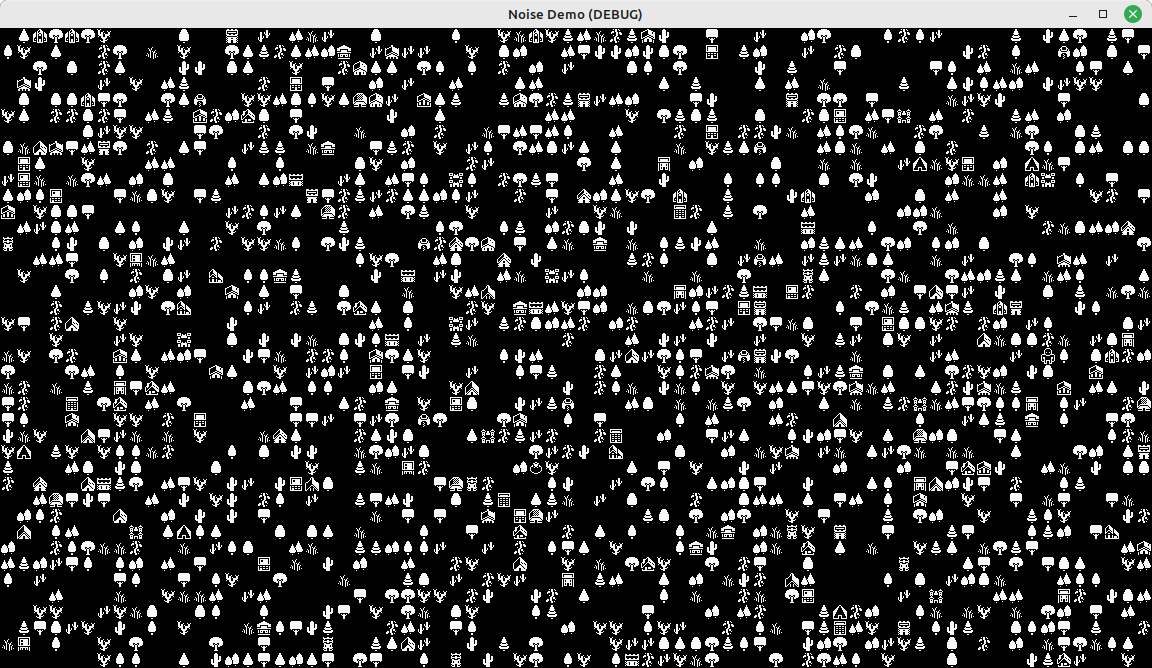
\includegraphics[width=\textwidth]{Images/simplex_smooth_default_1.png}
    \caption{A level of our scenario generated in the Simplex Noise implementation, using all of the default values \hyperref[noisedefaults]{shown here}. The level took a total of 99 milliseconds to be made.}
    \label{fig:simplexsmoothdefault1}
\end{figure}

\begin{figure}[H]
    \centering
    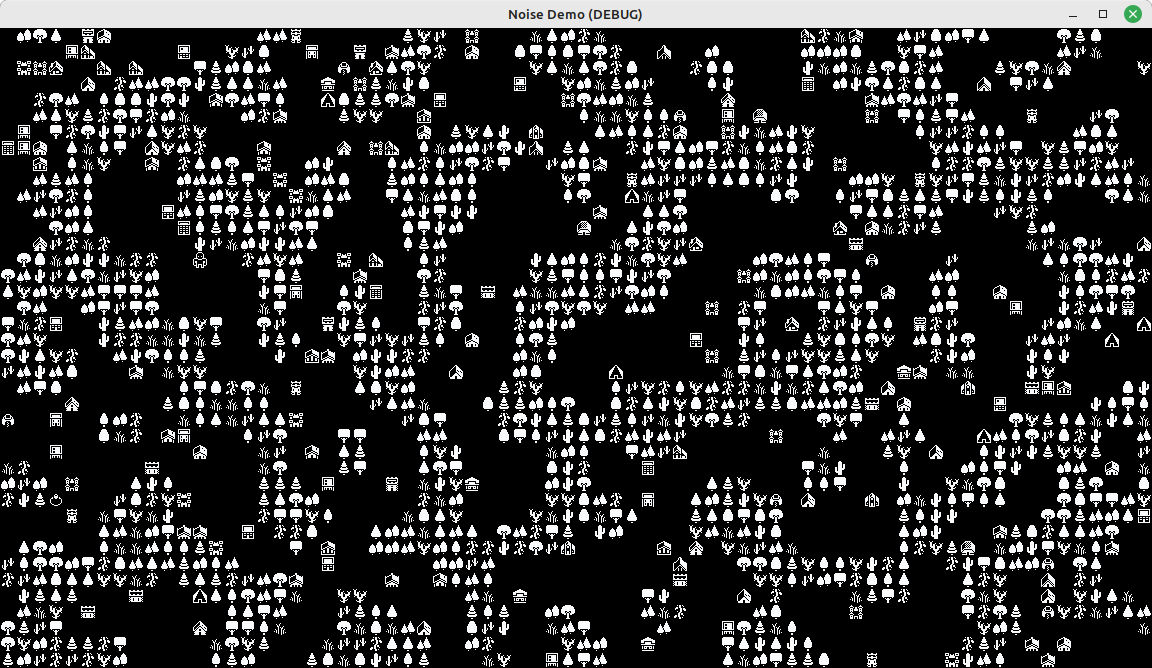
\includegraphics[width=\textwidth]{Images/simplex_smooth_0.01_frequency.png}
    \caption{A level of our scenario generated in the Simplex Noise implementation, setting the noise frequency to 0.01 (the default value for noise frequency in ``FastNoiseLite") and using the rest of the defaults \hyperref[noisedefaults]{shown here}. The level took a total of 104 milliseconds to be made.}
    \label{fig:simplexsmooth0.01}
\end{figure}

The 
\chapter{Implementation} \label{Implementation}

% Go deeper into how I got each algorithm to work
% How I decide

Here I will go a degree deeper as to how I made each algorithm work. Where possible, I plan to use code snippets from the work I have done to justify how and why things were implemented the way they were.

\section{Lindenmayer System} \label{implsys2}

To implement our basic grammar in Godot (see chapter \ref{lbasic}), we can take each rule and replace each string in accordance to our one rule, using the replace method, as demonstrated in Figure \ref{fig:lsystem1}.

For handling more than one rule, we can instead use a new string buffer variable where, for each character in our string, we can attain a new string and append it to our string buffer. The resulting string is then returned and interpreted. This can be represented in Godot as demonstrated in Figure \ref{fig:lsystem2}, which uses two functions to perform string replacement. The first function \verb|get_new_replacement| performs the character replacement according to the L-System's grammar rules, while the second function \verb|replace_string| uses a string builder variable to allow for replacement of characters without directly affecting the original string and causing unwanted side effects (see chapter \ref{implsys1} and also the tutorial in the following citations\cite{codatGD3LSystemYT}\cite{codatGD3LSystemGH}\cite{codatGD4LSystemGH}, from which I took major inspiration for my L-System implementation). The \verb|get_new_replacement| function was eventually used in my final implementation, whereas the code in the \verb|replace_string| function was adapated into my implementation's \verb|parse| function, shown in Figure \ref{fig:lsystem5}, in which some export variables were accounted for and the number of iterations was controlled through a while loop rather than a for loop, the while condition being that the string size was smaller than the total number of cells. The string that \verb|parse| returns chops off any excess characters.

This can \textit{then} be used to handle more complex grammars that can handle more than one rule in which characters in strings are replaced by other strings of variable length, as seen in the example in Chapter \ref{lcomplex}.

With a constant use of the same grammar rules and axiom, one issue that arose in the development of levels in our scenario, with L-Systems, is the lack of variance in the kinds of tiles placed, and it was hard to figure out how to deviate even slightly from the eventually recognisable patterns the algorithm and default grammar (see chapter \ref{implsys1}) would create. I thus developed a mitigation for this by allowing a choice between the provided axiom or a random one (the user/developer can also change the axiom in Godot's editor). This is down to the exported variables in the L-System node's script that I implemented (the L-System node's parent is the \verb|TileMap| root node). The relevant ones from the \verb|l_system.gd| script file are shown in Figure \ref{fig:lsystem3}. If \verb|use_random_axiom| is set to true (and it is by default), then it takes a maximum character limit \verb|upper_limit| (again an export variable configurable in the Godot editor itself) and then it generates a string of a length \textbf{up to} that limit- that is, the length of the returned string between 1 and the limit, both inclusive- using the alphabet that all of the provided grammars adhere to (``O" for blank space, ``W" for trees and ``B" for buildings). The axiom is then assigned to the \verb|string| script variable in the \verb|paint| method by calling the \verb|paint| method and assigning the return type to it.

For the sake of creativity and additional experimentation, I created additional grammars that can be configured with the \verb|ruleset| variable. The ``Default" grammar is as described in \ref{implsys1}, and the additional grammars generate higher proportions of either buildings, trees or empty space depending on which one is chosen (with the ``more buildings" grammar producing levels that are impossible to finish in our scenario). The grammars themselves are detailed in Figure \ref{fig:lsystem4}, and the method used to return the specifically set grammar in \verb|parse| is shown in Figure \ref{fig:lsystem6}.

\begin{figure}[H]
    \centering
    \begin{lstlisting}
string = string.replace(rule["from"], rule["to"]) #Here the rules were stored in dictionaries.
    \end{lstlisting}
    \caption{A line of code that demonstrates directly replacing characters in a string according to our L-System grammar's rules.}
    \label{fig:lsystem1}
\end{figure}

\begin{figure}[H]
    \centering
    \begin{lstlisting}
func get_new_replacement(character: String) -> String:
	for rule in rules:
		if rule["from"] == character:
			return rule["to"]
	return character

func replace_string(string: String) -> String:
	var new_string = ""
	for character in string:
		new_string += get_new_replacement(character)
	return new_string
    \end{lstlisting}
    \caption{Two GDScript functions for replacing characters in an L-System grammar with more than one rule. The first function was used in the final L-System implementation of the scenario. The second function was adapted into the ``parse" function of my implementation. Both functions are in the l\_system.gd script file.}
    \label{fig:lsystem2}
\end{figure}

\begin{figure}[H]
    \centering
    \begin{lstlisting}
@export var use_random_axiom: bool = true
## Defines how many characters a random axiom can have MAXIMUM. Only used when use_random_axiom is true.
@export var upper_limit: int = 10
    \end{lstlisting}
    \caption{The use\_random\_axiom and upper\_limit variables used when allowing a random axiom for an L-System grammar and then setting a maximum character limit for it.}
    \label{fig:lsystem3}
\end{figure}

\begin{figure}[H]
    \centering
    $$ \mbox{O} \rightarrow \mbox{B}\mbox{W}\mbox{O}\mbox{B} $$
    $$ \mbox{W} \rightarrow \mbox{W}\mbox{B}\mbox{O}\mbox{B}\mbox{O} $$
    $$ \mbox{B} \rightarrow \mbox{B}\mbox{B} $$
    
    $$ \mbox{O} \rightarrow \mbox{W}\mbox{W}\mbox{O} $$ 
    $$ \mbox{W} \rightarrow \mbox{W}\mbox{B}\mbox{W}\mbox{O} $$
    $$ \mbox{B} \rightarrow \mbox{B}\mbox{W}\mbox{W}\mbox{O} $$
    
    $$ \mbox{O} \rightarrow \mbox{O}\mbox{O}\mbox{B}\mbox{W}\mbox{O} $$ 
    $$ \mbox{W} \rightarrow \mbox{O}\mbox{B} $$
    $$ \mbox{B} \rightarrow \mbox{O}\mbox{W} $$
    \caption{The other 3 grammars I created for my L-System implementation, aside from the default one covered in chapter \ref{implsys1}. More buildings, more trees and more space respectively.}
    \label{fig:lsystem4}
\end{figure}

\begin{figure}[H]
    \centering
    \begin{lstlisting}
func _size() -> int:
	return tile_map.x_tile_range * tile_map.y_tile_range

func rand_axiom() -> String:
	var string_buffer: String = ""
	var limit: int = randi_range(1, upper_limit)
	for i in range(limit):
		string_buffer += ["O", "W", "B"].pick_random()
	return string_buffer
 
func parse() -> String:
	if use_random_axiom:
		axiom = rand_axiom()
		string = axiom
	if not use_custom_ruleset or ruleset != "Default":
		rules = _get_ruleset()
	var size: int = _size()
	while len(string) <= size:
		var new_string = ""
		for character in string:
			new_string += get_new_replacement(character)
		string = new_string
	string = string.substr(0, size)
	return string
    \end{lstlisting}
    \caption{The parse function in l\_system.gd, which takes the rand\_axiom and \_get\_ruleset functions (if needed; the latter is shown in Figure \ref{fig:lsystem6}), then gets the string size through \_size. Then, the string replacements described in \ref{fig:lsystem2} are carried out in the while loop, before the string is then returned (albeit without any excess characters that will not be used in the paint method to paint the cells in the tile map).}
    \label{fig:lsystem5}
\end{figure}

\begin{figure}[H]
    \centering
    \begin{lstlisting}
func _get_ruleset() -> Array[Dictionary]:
	match ruleset:
		"More Buildings (IMPOSSIBLE)": return MORE_BUILDINGS
		"More Trees": return MORE_TREES
		"More Space": return MORE_SPACE
		_: return DEFAULT
    \end{lstlisting}
    \caption{The \_get\_ruleset function used in the parse method in figure \ref{fig:lsystem5}.}
    \label{fig:lsystem6}
\end{figure}

\section{Perlin/Simplex Noise} \label{impperlin2}

While the \verb|noise_type| export variable is a selection of strings that are eventually taken from to return an enumeration for \verb|NoiseType|, a member of the \verb|FastNoiseLite| class\cite{fastnoiselitedocs}, the \verb|fractal_type| and \verb|cellular_distance_type| export variables more directly correspond to the relevant enumerations from \verb|FastNoiseLite|, as described earlier in chapter \ref{impperlin1} and shown in Figure \ref{fig:simplex1}. The \textit{other} export variable is \verb|noise_frequency|, which corresponds to the \verb|frequency| property in \verb|FastNoiseLite|. This is again shown in Figure \ref{fig:simplex1}.

Initiating the noise variable is done in the \verb|set_noise| function, in which, after instantiating the \verb|FastNoiseLite| class, the relevant export variables are then taken in and assigned their values accordingly, with the noise type handled through the \verb|_get_noise_type| function, which returns an integer that is then cast to the \verb|NoiseType| enumeration. By contrast, all the other attribute assignments- \verb|frequency|, \verb|fractal_type| and \verb|cellular_distance_function|- were far more simple, since I could just use the values of \verb|noise_frequency|, \verb|fractal_type| (\textit{in the script's export variable, \textbf{not} the noise instance}) and \verb|cellular_distance_type|, and assign them accordingly. Both functions are shown in Figure \ref{fig:simplex2}.

In both Figures \ref{fig:simplex1} and \ref{fig:simplex2}, I had a commented out export variable, \verb|octaves|. I wanted to see if changing the number of octaves in our noise image (or, rather, ``layers") would have an effect on the level layouts designed (the default is 5\cite{fastnoiselitedocs}). Unfortunately, in my experiments, I found that it did not have any noticeable effect, so I decided to leave the default number of octaves as is. 

Painting the tiles in our tile map involves a \verb|paint_points| method in which we iterate through every single cell of our tile map. For each cell in that map, we then check first if it can paint a tree. If the noise value retrieved at the given pixel from the noise image is smaller than the maximum limit we set for trees, \verb|tree_cap|, then we paint a tree tile at that cell. Then, we check for buildings. As I described in chapter \ref{impperlin1}, I had to implement additional Boolean checks for when \verb|tree_cap| was smaller than \verb|building_cap|, so that buildings could still get placed. First, we check that \verb|building_cap| is smaller than \textit{or equal to} \verb|tree cap| \textbf{and}, if so, whether or not we overwrite the tree tile with a building tile in the same place, subject to a random float between 0 and 1 falling below the probability value set in \verb|building_overtakes_tree|. The \textit{alternative}, for when \verb|building_cap| is smaller than \verb|tree_cap|, is to check whether the current \verb|noise_point| is smaller than the \verb|building_cap| we set. In both cases, of course, that cell cannot already be occupied by something else. If those conditions are true, we can then paint a building tile. The code behind this part of the algorithm is shown in Figure \ref{fig:simplex3}.

\begin{figure}[H]
    \centering
    \begin{lstlisting}
var noise: FastNoiseLite
@export_enum("Perlin", "Simplex", "Simplex Smooth", "Value", "Value Cubic") var noise_type: String = "Simplex Smooth"
@export var fractal_type: FastNoiseLite.FractalType
@export var cellular_distance_type: FastNoiseLite.CellularDistanceFunction
#@export_range(1, 10, 1) var octaves: int = 5 
@export_range(0.0, 1.0) var noise_frequency: float = 0.894
    \end{lstlisting}
    \caption{The noise, noise\_type, fractal\_type, cellular\_distance\_type and noise\_frequency script variables in tile\_map.gd. The latter three are export variables, and the latter two of \textit{those} are assigned to the enumerations FractalType and CellularDistanceFunction repsectively (both are members of the FastNoiseLite class).\cite{fastnoiselitedocs} noise\_type, meanwhile, uses an external function called to assign properties to a newly created FastNoiseLite instance which is assigned to the noise script variable. noise\_frequency here corresponds to the frequency attribute in FastNoiseLite.\\Notice the commented out octaves variable. Changing the number of octaves used had no effect on the level layouts produced, so I left the default number of octaves (5) as is.}
    \label{fig:simplex1}
\end{figure}

\begin{figure}[H]
    \centering
    \begin{lstlisting}
func _get_noise_type() -> int:
	match noise_type:
		"Perlin": return 3
		"Simplex": return 0
		"Value": return 5
		"Value Cubic": return 4
		_: return 1 # Return Simplex Smooth by default

func set_noise() -> void:
	noise = FastNoiseLite.new()
	noise.frequency = noise_frequency
	noise.noise_type = _get_noise_type() as FastNoiseLite.NoiseType
	noise.fractal_type = fractal_type
	noise.cellular_distance_function = cellular_distance_type
#	noise.fractal_octaves = octaves
	noise.seed = randi()
    \end{lstlisting}
    \caption{The set\_noise method in the tile\_map.gd script, which uses the earlier defined \_get\_noise\_type method to assign the noise type. The noise type returned is then cast from an integer to an enumeration of type NoiseType (from FastNoiseLite). The fractal\_octaves line is commented out because, when experimenting with octaves, I found no real effects they could have on the level layouts generated, so I left the default number of octaves (5) as is.}
    \label{fig:simplex2}
\end{figure}

\begin{figure}[H]
    \centering
    \begin{lstlisting}
func paint_tiles() -> void:
	for x in range(x_tile_range):
		for y in range(y_tile_range):
			var noise_point: float = noise.get_noise_2d(x * tile_set.tile_size.x, y * tile_set.tile_size.y)
			if noise_point < tree_cap and not get_used_cells(0).has(Vector2i(x, y)):
				set_cell(0, Vector2i(x, y), 0, trees.pick_random())
			if ((building_cap <= tree_cap and randf() < building_overtakes_tree) or (building_cap > tree_cap and noise_point < building_cap)) and not get_used_cells(0).has(Vector2i(x, y)):
				set_cell(0, Vector2i(x, y), 0, buildings.pick_random())
    \end{lstlisting}
    \caption{The paint\_tiles method in the tile\_map.gd script iterates through the tile map and gets each noise pixel from the relevant part of the noise image. It first tries to paint a tree tile there, subject to the noise\_point value being below the limit set for trees. Then, it decides whether or not to paint a building there. The conditions for painting building tiles are as described in chapter \ref{impperlin1} and further elaborated on earlier in \textit{this} chapter, \ref{impperlin2}.}
    \label{fig:simplex3}
\end{figure}

\section{Poisson Disk Sampling}

To be able to access the inner and outer grid sizes in my implementation of this algorithm, since GDScript does not have a concept of different \verb|Array|s and lists, I stored the lengths of the inner and outer grid in local variables in the \verb|generate_points| function. Those local variables, \verb|grid_x_axis_size| and \verb|grid_y_axis_size| as shown in Figures \ref{fig:pds1} and \ref{fig:pds2}, essentially store the same grid size values as in Lague's implementation, right down to performing the same division in a ceiling function, to the inner grid and the outer grid respectively. Since these dimensions would also be needed for \verb|is_valid|, instead of creating 2 more script variables, I instead took them in as 2 additional method parameters, as shown in Figures \ref{fig:pds3} and \ref{fig:pds4}, and used them accordingly when calculating the maximum and minimum bounds for searching the nearest points of the cell, as shown in \ref{fig:pds5}. Doing it this way ensured that the computation of this algorithm would stay efficient and not stall with an adequate (not too high) number of rejection samples.

\begin{figure}[H]
    \centering
    \begin{lstlisting}
var grid_x_axis_size: int = ceili(sample_region_size.x/cell_size)
var grid_y_axis_size: int = ceili(sample_region_size.y/cell_size)
    \end{lstlisting}
    \caption{The lines used to determine the inner and outer dimensions of the grid array.}
    \label{fig:pds1}
\end{figure}

\begin{figure}[H]
    \centering
    \begin{lstlisting}
for i in range(grid_x_axis_size):
	grid.append([])
	for j in range(grid_y_axis_size):
		grid[i].append(0)
    \end{lstlisting}
    \caption{The nested for-loop that initialises the grid array. First, each inner array is initialised and inserted, then a number of zeroes, determined by the grid's y-dimension, are inserted.}
    \label{fig:pds2}
\end{figure}

\begin{figure}[H]
    \centering
    \begin{lstlisting}
if is_valid(candidate, sample_region_size, cell_size, radius, points, grid, grid_x_axis_size, grid_y_axis_size):
    \end{lstlisting}
    \caption{The line that uses the grid's x and y dimensions as parameters. This calls the is\_valid method using those additional parameters (see Figure \ref{fig:pds4}).}
    \label{fig:pds3}
\end{figure}

\begin{figure}[H]
    \centering
    \begin{lstlisting}
func is_valid(candidate: Vector2, sample_region_size: Vector2, cell_size: float, radius: float, points: Array[Vector2], grid: Array[Array], grid_x_axis_size: int, grid_y_axis_size: int) -> bool
    \end{lstlisting}
    \caption{The function is\_valid, which takes in 2 additional parameters denoting the x and y dimensions of the grid array used in generate\_points.}
    \label{fig:pds4}
\end{figure}

\begin{figure}[H]
    \centering
    \begin{lstlisting}
var search_end_x: int = min(cell_x + 2, grid_x_axis_size - 1)
var search_end_y: int = min(cell_y + 2, grid_y_axis_size - 1)
    \end{lstlisting}
    \caption{The relevant lines of code in is\_valid that reference the grid's x and y dimensions, stored in additional variables as aforementioned.}
    \label{fig:pds5}
\end{figure}

\section{Voronoï Cells}

The original JavaScript implementation, as mentioned before, had a \verb|randRange| function that I took out, but there was also an additional \verb|mapSize| parameter in \verb|definePoints| that, in \textit{my} \verb|define_points| function, didn't really need, since I made sure the map's dimensions were readily accessible via the \verb|x_tile_range| and \verb|y_tile_range| script variable. I therefore took out the second parameter in \verb|define_points|, as shown in Figure \ref{fig:voronoi1}, and substituted it with \verb|x_tile_range| and \verb|y_tile_range| accordingly, as shown in Figure \ref{fig:voronoi3}.

The type of each Voronoï cell was determined by taking, and then deleting, a value from the \verb|types| array. Said array is local to that function, and it is initialised by duplicating the \verb|trees| array, then appending it with the \verb|buildings| array, making sure the same type cannot be used for a Voronoï cell twice. Duplicating the array before merging it essentially makes sure that the \textit{original} \verb|trees| array is not affected by deletions performed on the \verb|types| array. This computation is shown in Figure \ref{fig:voronoi2}, and the deletion operation is shown in Figure \ref{fig:voronoi4}.

Another addition to my implementation of the algorithm was the choice of using either the Euclidean distance or Manhattan distance for calculating the distance between points that would form cells. This was done with a function \verb|calculate_points_delta|, as shown in Figure \ref{fig:voronoi9} and used in Figure \ref{fig:voronoi8}, which is called on the calculation of \verb|delta| in \verb|define_points|. The function takes the contents of the exported variable \verb|distance|, as well as the current \verb|x| and \verb|y| coordinates and point ID \verb|p| during the current points delta calculation. It then checks if the String value in \verb|distance| denotes either the Euclidean distance or the Manhattan distance, then it finally returns the appropriate calculation. Using the Manhattan distance instead of the Euclidean distance does indeed yield a considerable performance increase (as well as creating fewer Voronoï cells by using a smaller \verb|random_starting_points| value), which I touch on in the Evaluation chapter.

Furthermore, my implementation would often paint cells in the tile map that were out of bounds, so to mitigate this when painting them, I created an additional function \verb|_is_in_bounds|, as shown in Figure \ref{fig:voronoi7} and used in Figure \ref{fig:voronoi6}, for checking whether a painted cell (that is, the coordinates of the current point \textbf{plus} the delta/difference between it and the closest of the randomly selected starting points to it) is within the boundaries of the tile map. If it is not, then it does not get painted, though it is not deleted from the point's citizens array either.

\begin{figure}[H]
    \centering
    \begin{lstlisting}
func define_points(num_points: int) -> void:
    \end{lstlisting}
    \caption{The define\_points function header, with no argument for the map's size. The num\_points value that gets taken in during runtime is determined by the script's export variable random\_starting\_points.}
    \label{fig:voronoi1}
\end{figure}

\begin{figure}[H]
    \centering
    \begin{lstlisting}
var types: Array[Vector2i] = trees.duplicate()
types.append_array(buildings)
    \end{lstlisting}
    \caption{The types array being initialised in define\_points, with its values taken from the trees and buildings arrays, such that no type can be used for a cell twice, while also making sure that the original trees and buildings arrays are not affected by the deletions on types.}
    \label{fig:voronoi2}
\end{figure}

\begin{figure}[H]
    \centering
    \begin{lstlisting}
var x: int = randi_range(0, x_tile_range)
var y: int = randi_range(0, y_tile_range)
    \end{lstlisting}
    \caption{Godot's built-in randi\_range function being used in place of a self-defined one in define\_points.}
    \label{fig:voronoi3}
\end{figure}

\begin{figure}[H]
    \centering
    \begin{lstlisting}
var type: Vector2i = types.pick_random()
types.erase(type)
    \end{lstlisting}
    \caption{The types of each Voronoï cell being picked and the erased in define\_points.}
    \label{fig:voronoi4}
\end{figure}

\begin{figure}[H]
    \centering
    \begin{lstlisting}
const EUCLIDEAN: String = "Euclidean distance"
const MANHATTAN: String = "Manhattan distance"
@export_enum(EUCLIDEAN, MANHATTAN) var distance: String = MANHATTAN
    \end{lstlisting}
    \caption{The applicable values of the exported variable distance.}
    \label{fig:voronoi5}
\end{figure}

\begin{figure}[H]
    \centering
    \begin{lstlisting}
if _is_in_bounds(point["x"], citizen["dx"], point["y"], citizen["dy"]):
    set_cell(0, Vector2(point["x"] + citizen["dx"], point["y"] + citizen["dy"]), 0, point["type"])
    \end{lstlisting}
    \caption{The appropriate block of code in the paint\_points function that checks to see if a point would be in bounds or out of bounds before painting it in its relevant tile map cell. It does \textbf{not} delete the point if it lies out of bounds.}
    \label{fig:voronoi6}
\end{figure}

\begin{figure}[H]
    \centering
    \begin{lstlisting}
func _is_in_bounds(x: int, dx: int, y: int, dy: int) -> bool:
	return x + dx >= 0 and x + dx < x_tile_range and y + dy >= 0 and  y + dy < y_tile_range
    \end{lstlisting}
    \caption{The \_is\_in\_bounds function called in the code snippet in Figure \ref{fig:voronoi6}.}
    \label{fig:voronoi7}
\end{figure}

\begin{figure}[H]
    \centering
    \begin{lstlisting}
func _squared(x: int) -> int:
	return x ** 2

func calculate_points_delta(x: int, y: int, p: int) -> float:
	if distance == EUCLIDEAN:
		return sqrt(_squared(points[p]["x"] - x) + _squared(points[p]["y"] - y))
	return abs(points[p]["x"] - x) + abs(points[p]["y"] - y)
    \end{lstlisting}
    \caption{The calculate\_points\_delta function being called in Figure \ref{fig:voronoi9}. \_squared is a self-defined helper function that is only used for the Euclidean distance calculation; it does as it says (it squares the number taken into it and returns the result).}
    \label{fig:voronoi8}
\end{figure}

\begin{figure}
    \centering
    \begin{lstlisting}
var delta: float = calculate_points_delta(x, y, p)
    \end{lstlisting}
    \caption{The calling of calculate\_points\_delta from Figure \ref{fig:voronoi8} in define\_points, using the current x and y coordinates and point ID p in the iteration when grouping tile map cells together to form Voronoï cells from the randomly selected starting points.}
    \label{fig:voronoi9}
\end{figure}
\chapter{Legal, Social, Ethical and Professional Issues} \label{Issues}
% Your report should include a chapter with a reasoned discussion about legal, social ethical and professional issues within the context of your project problem. You should also demonstrate that you are aware of the regulations governing your project area and the Code of Conduct \& Code of Good Practice issued by the British Computer Society, and that you have applied their principles, where appropriate, as you carried out your project.

\section{Using Other People's Resources}

Throughout my project, I made sure the resources I worked with were freely available to use in an academic context like this.
For example, the Unity tutorial I used as an inspiration of my Godot Poisson Disk Sampling implementation\cite{seblaguetuteYT} has its project files under the MIT License\cite{seblaguetuteGH}, a permissive open-source license which means it can be freely used and adapted with, even commercially.
The JavaScript code example I used from the Procedural Content Generation wiki, for my Voronoi Cells implementation, was submitted by an anonymous Wikidot contributor in 2017 and, like most if not all of the Wiki's contents, is licensed under the Creative Commons Attribution-ShareAlike 3.0 License; that is, the article and its contents (including the JavaScript code example) can be freely used and adapted, subject to the condition that the original source is attributed \textbf{and} that any transformed work, \textit{like my implementation}, \textbf{must} be published under the same or a compatible license. Since there are no listed compatible source code licenses I can use in lieu of this license, I must therefore abide by the license contents of the original article in my source code, since my implementation and the original JavaScript code are similar to a noticeable, but not entirely like for like, degree.

\section{How I Will Release My Own Artefacts}

\chapter{Results \& Evaluation} \label{Evaluation}

Here, we will discuss how the implementations of the algorithms in our scenario were tested and ensured that they ran as they should.

\section{Software Testing}

Due to the nature of the project (being several implementations of a computer game), the testing behind this project has solely revolved around trial-and-error, messing around with the exported variables in the Godot editor to see how things worked and what configurations worked best for our scenario. This involved taking many screenshots of generated levels and examining things by eye, seeing how layouts compared across implementations.

Despite this, I decided to run some simple performance tests to see how long each algorithm ran. These tests took some of the custom export variables from the scene scripts and ran them several times, with an average time calculated to the nearest millisecond. For the Noise implementation, these tests are in tables \ref{fig:table1}, in which each noise algorithm was paired with each cellular distance function, and \ref{fig:table2}, in which each noise algorithm was paired with each fractal type.

\section{Comparing the Different Algorithms and Drawing Conclusions on Which Ones Are Best}

\subsection{Performance}

With the L-System implementation, there were no problems whatsoever running the game very quickly on my machine, and quickly got satisfactory results. The table in Figure \ref{fig:table3} shows that the processing times remained miniscule even as the length of the axiom increased.

While my Noise implementation was slower than my L-System implementation by a magnitude, it was still satisfactorily quick.

With Poisson Disk Sampling, the higher the number of rejection samples (that is, the higher the maximum number of times a cell was sampled before it was either accepted or ultimately rejected), the longer it took to generate a complete level layout, and even, due to the nature of the tile map compared to the algorithm's \textit{usual} use (of scattering dots on a plane), it was not maximal (not all points had cells painted for them; some cells had their tiles overwritten as well). Using 8 rejection samples was usually enough to yield a satisfactory level layout while also keeping level creation times to a minimum.

Voronoï Cells took the longest to compute on average. Computations with the Euclidean distance measurement took longer than those measured with the Manhattan distance.

\subsection{Layouts}

Of the 4 implementations that were made for this project, the Noise and Poisson Disk Sampling implementation were by far the most similar, followed by the L-System implementation, and then the Voronoï Cells implementation, which was far and away the most unique.

While the noise implementations varied greatly depending on what settings were used, and the way the implementation was designed allowed for very many possibilities as to how the noise would turn out (and how it would affect the final level), the results that I found produced the most similar results to that of the Poisson Disk Sampling implementation had the following configurations:

\begin{itemize} \label{noisedefaults}
    \item Noise Type (``noise\_type"): Simplex Smooth
    \item Fractal Type (``fractal\_type"): Fractal None
    \item Cellular Distance Type/Function (``cellular\_distance\_type"): Distance Euclidean
    \item Noise Frequency (``noise\_frequency"): 0.894
    \item Tree Cap (``tree\_cap"): -0.048
    \item Building Cap (``building\_cap"): -0.252
    \item Building Overtakes Tree (``building\_overtakes\_tree"): 0.12
\end{itemize}

The default noise frequency in ``FastNoiseLite" is 0.01, which results in smoother and less disparate noise. As seen in Figure \ref{fig:simplexsmooth0.01}, the smoother noise and lower frequency results in a distinct kind of level layout in which represents some of the noise values in the image very clearly, such that tiles (both buildings and trees) are bunched together in partially interconnected groups, forming long, large lines of painted tiles. To describe this as best as possible, it is easy to discern that the level layout was determined from a noise image. Using a higher noise frequency to produce rougher noise, and more disparate level layouts, yields results like in Figure \ref{fig:simplexsmoothdefault1}, which makes it very similar to the layouts yielded in my Poisson Disk Sampling implementation and, to a lesser extent, my L-System implementation. While I personally like the former kind of level layout, part of the aim of this project was to compare in terms of which could produce the most similar, and, compared to the L-System and Poisson Disk Sampling implementations, the Noise implementation with the frequency set to 0.01 was far too distinct, hence the want to change it up.

\begin{figure}[H]
    \centering
    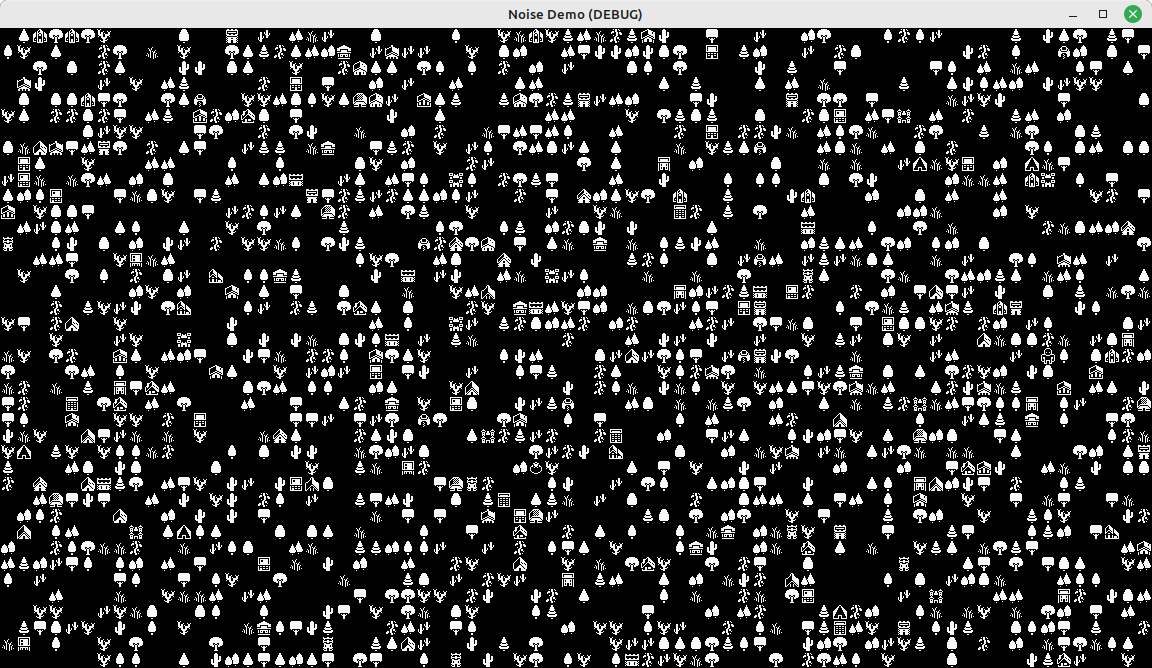
\includegraphics[width=\textwidth]{Images/simplex_smooth_default_1.png}
    \caption{A level of our scenario generated in the Simplex Noise implementation, using all of the default values \hyperref[noisedefaults]{shown here}. The level took a total of 99 milliseconds to be made.}
    \label{fig:simplexsmoothdefault1}
\end{figure}

\begin{figure}[H]
    \centering
    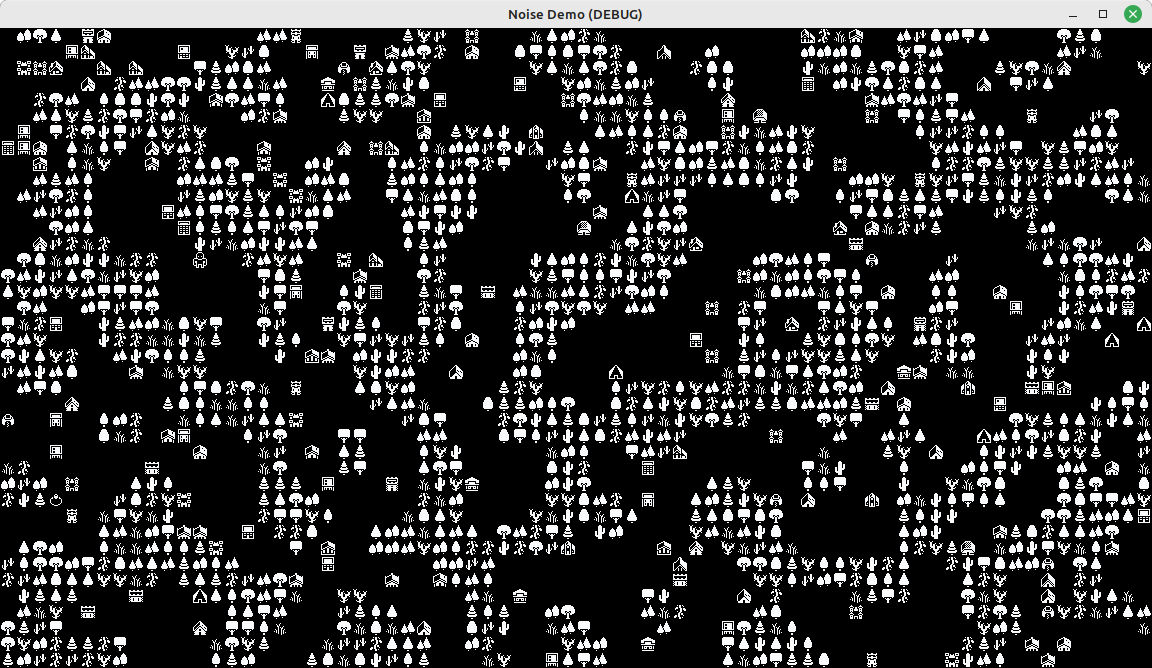
\includegraphics[width=\textwidth]{Images/simplex_smooth_0.01_frequency.png}
    \caption{A level of our scenario generated in the Simplex Noise implementation, setting the noise frequency to 0.01 (the default value for noise frequency in ``FastNoiseLite") and using the rest of the defaults \hyperref[noisedefaults]{shown here}. The level took a total of 104 milliseconds to be made.}
    \label{fig:simplexsmooth0.01}
\end{figure}

The 
\chapter{Conclusion and Future Work} \label{Conclusion}

% The project's conclusions should list the key things that have been learnt as a consequence of engaging in your project work. For example, ``The use of overloading in C++ provides a very elegant mechanism for transparent parallelisation of sequential programs'', or ``The overheads of linear-time n-body algorithms makes them computationally less efficient than $O(n \log n)$ algorithms for systems with less than 100000 particles''. Avoid tedious personal reflections like ``I learned a lot about C++ programming...'', or ``Simulating colliding galaxies can be real fun...''. It is common to finish the report by listing ways in which the project can be taken further. This might, for example, be a plan for turning a piece of software or hardware into a marketable product, or a set of ideas for possibly turning your project into an MPhil or PhD.

To conclude, I have gained a wealth of knowledge about the way some of the most popular procedural content generation algorithms work, and how they are typically integrated into working games. I also learnt how I could leverage the features of the Godot game engine for some of them; for example, the ``FastNoiseLite" class allows me to generate noise textures in Value, Perlin and even Simplex noise and then mpdify them accordingly with additional frequency settings, fractal types and cellular distance functions. By implementing them in my own 2D tiled RPG scenario, I was able to get 4 procedural generation algorithms well-integrated into working games, proving Godot's technical proficiency in making these kinds of games work, and proving my own abilities as a games programmer. I was also able to compare the implementations of my algorithms in such a way that the differences, in terms of both performance times and the kinds of levels they produced, could very easily be discerned. The motives of this project can be pushed still further by measuring and comparing the performances of these algorithms in Big-O notation, including even more ontogenic algorithms such as Worley Noise, the Diamond-Square algorithm, Markov Chains and Cellular Automata, as well as telelogical algorithms such as the Rain Drop algorithm and Reaction-Diffusion systems, using a larger tile map on all of these algorithms and even using a different, more intensive scenario entirely, such as a 3D walking simulator/open-world game. With procedural generation for level design, the possibilites are practically endless.

%%%%%%%%%%%%%%%%%%%%%%%%%%%%%%%%%
% References
%%%%%%%%%%%%%%%%%%%%%%%%%%%%%%%%%
\bibliographystyle{plain}
\bibliography{Bibliography/reference}
\addcontentsline{toc}{section}{Bibliography}

%%%%%%%%%%%%%%%%%%%%%%%%%%%%%%%%%
% Appendices
%%%%%%%%%%%%%%%%%%%%%%%%%%%%%%%%%
\appendix
\include{Appendices/appendix}
\chapter{User Guide} \label{Guide}
% You must provide an adequate user guide for your software. The guide should provide easily understood instructions on how to use your software. A particularly useful approach is to treat the user guide as a walk-through of a typical session, or set of sessions, which collectively display all of the features of your package. Technical details of how the package works are rarely required. Keep the guide concise and simple. The extensive use of diagrams, illustrating the package in action, can often be particularly helpful. The user guide is sometimes included as a chapter in the main body of the report, but is often better included in an appendix to the main report.

\section{Opening Godot}

To run the projects in the .zip file, extract the projects into one folder. Then open Godot 4 (all projects in the source code listings folder are Godot 4 projects, \textbf{not} Godot 3 projects). When you start Godot for the first time, the project manager should be completely empty, without any projects, as described in Figure \ref{fig:godot1}. Projects have to be imported either one-by-one (by clicking ``Import" and going to the relevant project and opening it) or by clicking "Scan", then going to a folder of Godot projects and selecting it. The projects can then be opened in the project manager and edited as needed in Godot. Click ``Scan", then go to the folder where you extracted the projects, then click the ``Select Current Folder" button, as shown in Figure \ref{fig:godot2}, and all the projects should show up in the editor, as shown in Figure \ref{fig:godot3}. You can then double click on any one project (or click on it once and click the ``Edit" button) to open it in the Godot editor, an example of which is shown in Figure \ref{fig:godot4}. Alternatively, to run the project itself without opening the editor, using the currently saved values for exported script variables where appropriate, click on the project \textit{once} and click the ``Run" button.

\begin{figure}[H]
    \centering
    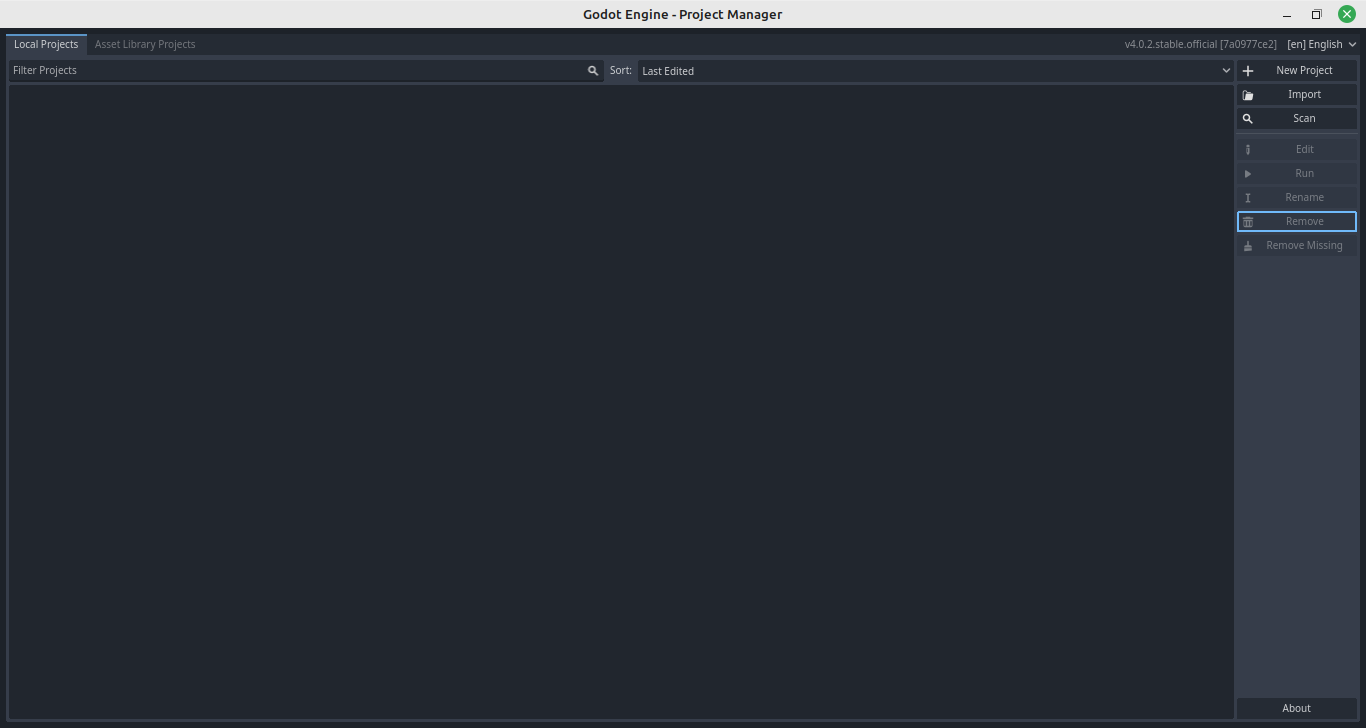
\includegraphics[width=\textwidth]{Images/open_godot.png}
    \caption{The Godot editor, when it is opened for the first time, does not show any projects in the editor (the Steam version bundles several example projects). Projects need to be imported either one-by-one or by scanning a folder of Godot projects.}
    \label{fig:godot1}
\end{figure}

\begin{figure}[H]
    \centering
    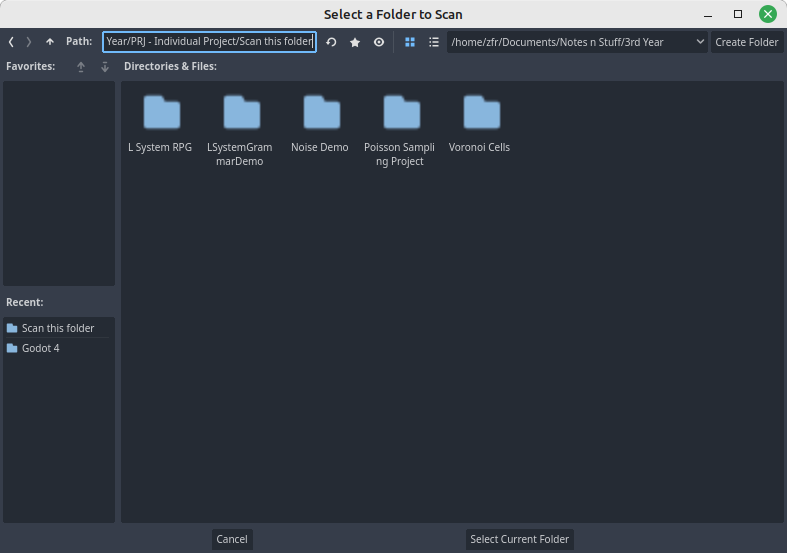
\includegraphics[width=\textwidth]{Images/scan-folder.png}
    \caption{You can click the "Scan" button in the project manager (in Figure \ref{fig:godot1}), then go to the relevant folder where your project are in Godot's built-in file explorer. Here, the artefacts behind this project have been exported into a separate folder called ``Scan this folder" as an example.}
    \label{fig:godot2}
\end{figure}

\begin{figure}[H]
    \centering
    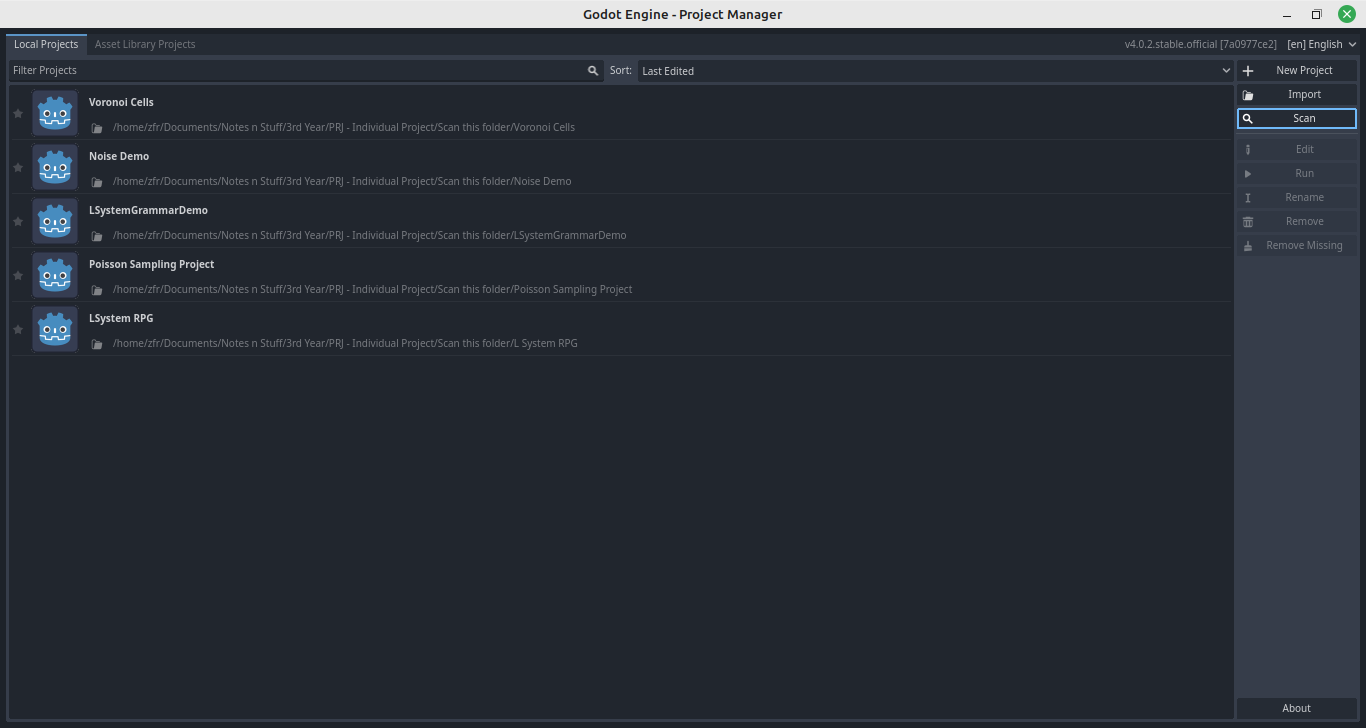
\includegraphics[width=\textwidth]{Images/projects-scanned.png}
    \caption{Once some Godot projects have been imported into the project manager, you should be able to easily view the list and double-click on any one of the projects to edit them, which will open the editor after closing the project manager. You could also click the ``Edit" button, or click ``Run" to run the game without having to open the editor itself.}
    \label{fig:godot3}
\end{figure}

\begin{figure}[H]
    \centering
    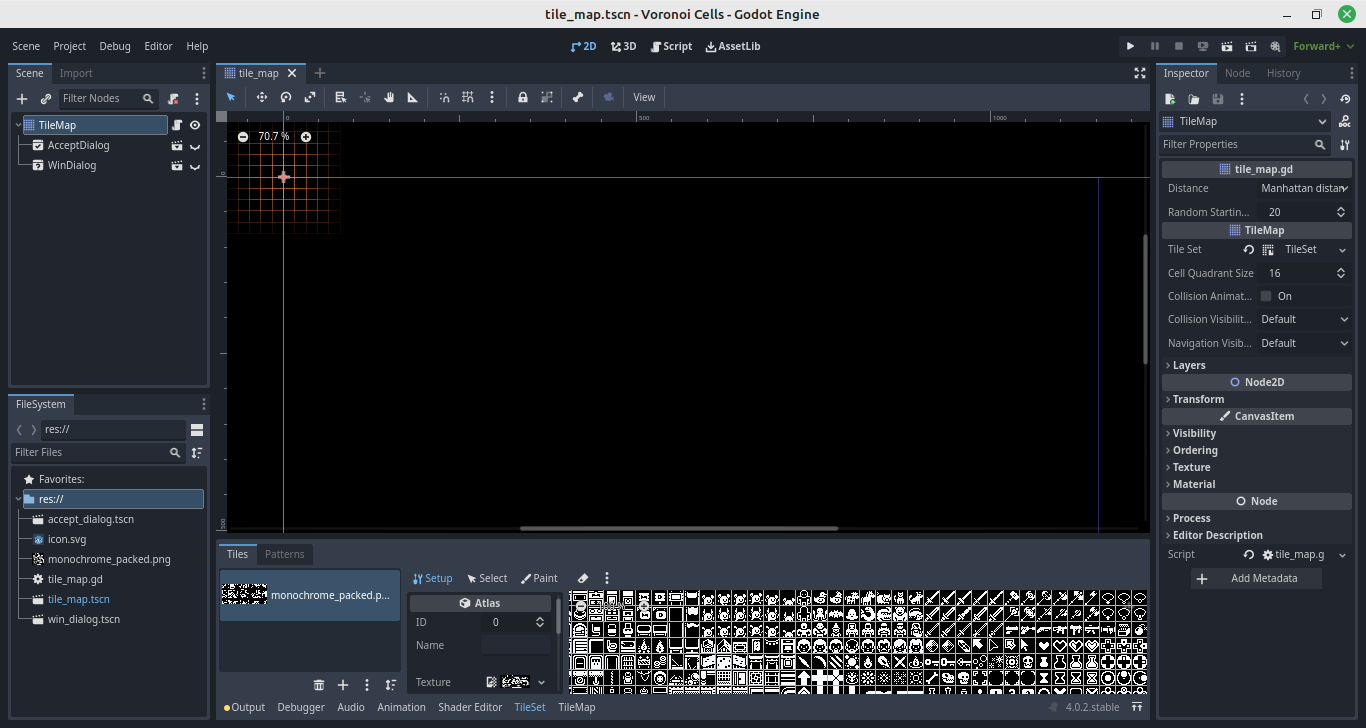
\includegraphics[width=\textwidth]{Images/godot-editor.png}
    \caption{The Godot editor open with the Voronoi cells project as an example. A visual description of the editor's contents is in chapter \ref{editor}.}
    \label{fig:godot4}
\end{figure}

\section{The Godot Editor} \label{editor}

As you open up the Godot editor, you will see the main scene view in the center, as shown in Figure \ref{fig:godot4}, using the Voronoi cells implementation as an example. The left-hand side shows the scene tree at the top, and the file system (from the root folder of the project) at the bottom. Meanwhile, the right hand side shows the currently selected node's export variables, \textit{including the custom export variables} defined in the node's script file, and two other tabs, ``Node" (which shows a list of signals for the scene that could be called in a script) and ``History" (which shows the sequence of recent actions performed on the scene during the current session). Above this is also a set of buttons which can be used for playing the project and/or the current scene. We go over how to run the current project in chapter \ref{runproject}.

\section{Custom Export Variables} 

When you click on some of the scenes in the projects, there may be some "exported" variables from scripts that are visible to you in the editor (examples include the "Distance" and "Random Starting Points" variables in the Voronoi Cells project). You can hover over the variable names in the editor and it will show a brief description of what the variable correlates to in the script. We will now go over the different export variables across all of the provided artefacts in this section.

\subsection{Lindenmayer System}

All of the custom export variables defined in scene scripts for your use are in the child node ``LSystem" (it is saved into its own scene file, but it is cheifly a child node of the root node ``TileMap"). Open the ``TileMap" scene (if it is not already opened for you when you launch the Godot editor) and click on the ``LSystem" node in the scene tree to edit it.

\begin{enumerate}
    \item axiom
    \begin{itemize}
        \item \textbf{Type:} String
        \item \textbf{Documentation:} The starting string from which the grammar starts applying its rules. Here it may be self defined, or randomly defined when ``use\_random\_axiom" is true.
        \item \textbf{Default value:} ``OWB"
    \end{itemize}
    \item use\_random\_axiom
    \begin{itemize}
        \item \textbf{Type:} Boolean (bool) 
        \item \textbf{Documentation:} Uses a random axiom with the currently set grammar, computed upon runtime, with a length up to (but not strictly) the value of upper\_limit. For example, if upper\_limit is set to 15, the generated axiom can be 15 characters, or it can be just 5 characters.
        \item \textbf{Default value:} true
    \end{itemize}
    \item upper\_limit
    \begin{itemize}
        \item \textbf{Type:} Integer (int)
        \item \textbf{Documentation:} Defines how many characters a random axiom can have MAXIMUM. Only used when ``use\_random\_axiom" is true.
        \item \textbf{Default value:} 10
    \end{itemize}
    \item use\_custom\_ruleset
    \begin{itemize}
        \item \textbf{Type:} Boolean (bool)
        \item \textbf{Documentation:} Allows the use of a customly defined ruleset made through amending the rules array in the editor.
        \item \textbf{Default value:} false
    \end{itemize}
    \item ruleset
    \begin{itemize}
        \item \textbf{Type:} String enumeration of the following choices:
        \begin{enumerate}
            \item ``Default"
            \item ``More Buildings (IMPOSSIBLE)"
            \item ``More Trees"
            \item ``More Space"
        \end{enumerate}
        \item \textbf{Documentation:} Denotes a series of pre-defined rulesets for this L-System grammar, of alphabet O (blank space), W (trees and fauna) and B (buildings), that can be chosen and then used on runtime. Can choose between a default ruleset, a ruleset that produces more buildings, a ruleset that produces more trees and a ruleset that produces more empty space.
        \item \textbf{Default value:} ``Default"
    \end{itemize}
    \item rules
    \begin{itemize}
        \item \textbf{Type:} Array of dictionaries
        \item \textbf{Documentation:} The set of rules that the L-System grammar uses. Shows the ``default" ruleset in the Godot editor for the user to see. If ``use\_custom\_ruleset" is set to true, this array can be edited with a custom defined ruleset that will be used on runtime, so long as it adheres to the alphabet of O (blank space), W (trees and fauna) and B (buildings).
        \item \textbf{Additional information:} The ``\_get\_ruleset" function uses the String value in ``ruleset" to set the value for ``rules" on runtime, \textit{if} ``use\_custom\_ruleset" is false (which it \textit{is} by default).
        \item \textbf{Default value:} The ``Default" grammar, as shown in Figure \ref{fig:defaultgrammar}.
    \end{itemize}
\end{enumerate}

\begin{figure}[H]
    \centering
    \begin{lstlisting}
    [
    	{
    		"from": "O",
    		"to": "OWO"
    	},
    	{
    		"from": "W",
    		"to": "WB"
    	},
    	{
    		"from": "B",
    		"to": "BWO"
    	}
    ]
    \end{lstlisting}
    \caption{The ``Default" grammar used for the ``rules" export variable, stored in the constant ``DEFAULT" in l\_system.gd. See l\_system.gd for the other grammars represented as arrays of dictionaries.}
    \label{fig:defaultgrammar}
\end{figure}

\subsection{Perlin/Simplex Noise}

\begin{enumerate}
    \item noise\_type
    \begin{itemize}
        \item \textbf{Type:} String enumeration of the following choices:
        \begin{enumerate}
            \item ``Perlin"
            \item ``Simplex"
            \item ``Simplex Smooth"
            \item ``Value"
            \item ``Value Cubic"
        \end{enumerate}
        \item \textbf{Documentation:} Defines the type of noise generation algorithm to use. Equates to the ``noise\_type" property in FastNoiseLite.
        \item \textbf{Default value:} ``Value Cubic"
    \end{itemize}
    \item fractal\_type
    \begin{itemize}
        \item \textbf{Type:} Enumeration of the following choices:
        \begin{enumerate}
            \item ``Fractal None"
            \item ``Fractal FBM"
            \item ``Fractal Ridged"
            \item ``Fractal Ping Pong"
        \end{enumerate}
        \item \textbf{Documentation:} Defines the type of method used to combine octaves of a noise image into a fractal. Directly equates to the FractalType enumeration in FastNoiseLite.
        \item \textbf{Default value:} ``Fractal None" 
    \end{itemize}
    \item cellular\_distance\_type
    \begin{itemize}
        \item \textbf{Type:} Enumeration of the following choices:
        \begin{enumerate}
            \item ``Distance Euclidean"
            \item ``Distance Euclidean Squared"
            \item ``Distance Manhattan"
            \item ``Distance Hybrid"
        \end{enumerate}
        \item \textbf{Documentation:} Defines the function used to calculate the distance between the nearest/second-nearest point(s). Directly equates to the CellularDistanceFunction enumeration in FastNoiseLite.
        \item \textbf{Default value:} ``Distance Euclidean"
    \end{itemize}
    \item noise\_frequency
    \begin{itemize}
        \item \textbf{Type:} Floating point number (float) between 0.0 and 1.0 inclusive
        \item \textbf{Documentation:} Defines the frequency of the generated noise, the higher the frequency, the rougher and more granular the noise.
        \item \textbf{Additional information:} The default value for ``frequency" in the ``FastNoiseClass" is 0.01, resulting in very smooth and distinct noise. 
        \item \textbf{Default value:} 0.894
    \end{itemize}
    \item tree\_cap
    \begin{itemize}
        \item \textbf{Type:} Floating point number (float) between -1.0 and 1.0 inclusive
        \item \textbf{Documentation:} Defines the upper limit to set for painting a tree tile on a specific noise pixel. If the value returned by the ``get\_noise\_2d" method (in FastNoiseLite) is smaller than this, then it gets painted.
        \item \textbf{Default value:} -0.048
    \end{itemize}
    \item building\_cap
    \begin{itemize}
        \item \textbf{Type:} Floating point number (float) between -1.0 and 1.0 inclusive
        \item \textbf{Documentation:} Defines the upper limit to set for painting a building tile on a specific noise pixel. If the value returned by the ``get\_noise\_2d" method (in FastNoiseLite) is smaller than this, then it gets painted. If the value of ``building\_cap" is smaller than ``tree\_cap," then decide whether or not to paint a building cell there with ``building\_overtakes\_tree."
        \item \textbf{Default value:} -0.252
    \end{itemize}
    \item building\_overtakes\_tree
    \begin{itemize}
        \item \textbf{Type:} Floating point number (float) between 0.0 and 0.5 inclusive
        \item \textbf{Documentation:} Only used when ``building\_cap" is smaller than ``tree\_cap." Determines the probability that a building tile would be painted in a cell where a tree tile was, or could be, also painted. Whether or not the cell actually is painted over is decided on computation time.
        \item \textbf{Default value:} 0.12
    \end{itemize}
\end{enumerate}

\subsection{Poisson Disk Sampling}

\begin{enumerate}
    \item paint\_building\_probability
    \begin{itemize}
        \item \textbf{Type:} Floating point number (float) between 0.0 and 1.0 inclusive
        \item \textbf{Documentation:} The probability that a building gets painted at a cell in lieu of a tree. The higher this probability, the more likely a building tile gets painted instead of a tree tile. 
        \item \textbf{Default value:} 0.125
    \end{itemize}
    \item point\_radius
    \begin{itemize}
        \item \textbf{Type:} Floating point number (float) between 0.5 and 2.5 inclusive
        \item \textbf{Documentation:} The radius value used to measure distances between points for the algorithm. The longer the radius, the further apart points are during the algorithm's processing, and the further apart painted cells are in the game.
        \item \textbf{Default value:} 1.0
    \end{itemize}
    \item region\_size
    \begin{itemize}
        \item \textbf{Type:} Vector2
        \item \textbf{Documentation:} The size of the region in which the algorithm is performed. Set to the "default" tile map size (72, 40) in the script, shown as (0, 0) in the Godot editor. Can be changed to use a smaller region for the algorithm itself, of course resulting in less cells covered within the boundaries set for this game, though the algorithm will perform faster due to less cells being checked.
        \item \textbf{Default value:} 
        \begin{itemize}
            \item \textbf{x}: The value in ``x\_tile\_range" (72)
            \item \textbf{y}: The value in ``y\_tile\_range" (40)
        \end{itemize}
    \end{itemize}
    \item rejection\_samples
    \begin{itemize}
        \item \textbf{Type:} Integer (int) between 1 andc 50 inclusive
        \item \textbf{Documentation:} The maximum number of times a cell is checked before it is ignored. A cell can be accepted and painted on before this maximum number is reached. The higher this value, the more times a cell is checked, therefore the higher the algorithm's processing time.
        \item \textbf{Default value:} 8
    \end{itemize}
\end{enumerate}

\subsection{Voronoï Cells}

\begin{enumerate}
    \item distance
    \begin{itemize}
        \item \textbf{Type:} String enumeration of the following choices:
        \begin{enumerate}
            \item ``Euclidean distance"
            \item ``Manhattan distance"
        \end{enumerate}
        \item \textbf{Documentation:} Determines whether or not the Euclidean or Manhattan distance formula is used for calculation of the deltas between points within Voronoi cells.
        \item \textbf{Default value:} ``Manhattan distance"
    \end{itemize}
    \item random\_starting\_points
    \begin{itemize}
        \item \textbf{Type:} Integer (int) between 15 and 40 inclusive
        \item \textbf{Documentation:} Determines the number of points randomly picked from at the start. Therefore, it also determines the number of cells in our Voronoi tesselation.
        \item \textbf{Default value:} 20
    \end{itemize}
\end{enumerate}

\subsection{The Basic L-System Demo Used to Create the Screenshots in Chapter \ref{alglsys}}

There is only one export variable for this: ``choices", which allows you to choose which one of the three provided rulesets to use. ``choices" is the default ruleset, and either ``deterministic" or ``basic" can be chosen. It is in the ``DemoNode" scene, the only scene of this Godot project. Quoting the documentation comment, this export variable ``Allows you to decide which ruleset to use. See the script file for the sources of said rulesets." The ruleset is assigned with the ``set\_values" function.

\newpage

\section{Running the Godot Projects} \label{runproject}

To \textit{run} the current project in the Godot editor, go to the bar above the Inspector, Node and History tabs on the right-hand side. You will find a \faPlay{} button which will play the main scene of the project (in my artefacts, the main scenes have already been set; if it were not already set, you would have been asked to set one). If closing the window to stop the project does not work, hit the \faStop{} button to end it. If you want to replay the current project without having to stop it, hit the \faPlay{} button again. Although \textbf{both} the icon \textbf{and} the colour of the \faPlay{} button will have changed by then, it will be in the same position as before.

As described in section \ref{commonalities}, only the close button of both the popup dialogs in the game seems to work properly for the moment, but this does not adversely affect the game functioning properly, nor does it adversely affect this project, so this is trivial.

\chapter{Source Code}
\section{Instructions}
Complete source code listings must be submitted as an appendix to the report. The project source codes are usually spread out over several files/units. You should try to help the reader to navigate through your source code by providing a ``table of contents'' (titles of these files/units and one line descriptions). The first page of the program listings folder must contain the following statement certifying the work as your own: ``I verify that I am the sole author of the programs contained in this folder, except where explicitly stated to the contrary''. Your (typed) signature and the date should follow this statement.

All work on programs must stop once the code is submitted to KEATS. You are required to keep safely several copies of this version of the program and you must use one of these copies in the project examination. Your examiners may ask to see the last-modified dates of your program files, and may ask you to demonstrate that the program files you use in the project examination are identical to the program files you have uploaded to KEATS. Any attempt to demonstrate code that is not included in your submitted source listings is an attempt to cheat; any such attempt will be reported to the KCL Misconduct Committee.

\textbf{You may find it easier to firstly generate a PDF of your source code using a text editor and then merge it to the end of your report. There are many free tools available that allow you to merge PDF files.}


\end{document}
